\documentclass[10pt, conference, letterpaper]{IEEEtran}
\IEEEoverridecommandlockouts
% The preceding line is only needed to identify funding in the first footnote. If that is unneeded, please comment it out.
\usepackage{cite}
\usepackage{amsmath,amssymb,amsfonts}
% \usepackage{amssymb}
\usepackage{graphicx}
\usepackage{textcomp}
\usepackage{xcolor}
\def\BibTeX{{\rm B\kern-.05em{\sc i\kern-.025em b}\kern-.08em
    T\kern-.1667em\lower.7ex\hbox{E}\kern-.125emX}}
\usepackage[linesnumbered,ruled,vlined]{algorithm2e}
\usepackage{subfigure}
\usepackage{flushend}

\usepackage{array}
\usepackage{multirow}

\usepackage[colorlinks=true, allcolors=black]{hyperref} % 添加这行

\hypersetup{bookmarks=false}

\newtheorem{definition}{\textbf{Definition}}
\newtheorem{theorem}{\textbf{Theorem}}
\setlength{\columnsep}{0.241 in}
\newcommand{\CLASSINPUTtoptextmargin}{0.75 in}
\newcommand{\CLASSINPUTbottomtextmargin}{1 in}
% \documentclass[a4paper,conference]{IEEEtran}
\usepackage[letterpaper, left=0.62 in, right=0.62 in, top=1.92cm,bottom=3.45cm]{geometry}
\begin{document}

% % Multi-stages Pareto-based Strategies of Edge Servers and Services\\
% %{\footnotesize \textsuperscript{*}Note: Sub-titles are not captured in Xplore and should not be used}
% %\thanks{Identify applicable funding agency here. If none, delete this.}
% }

\title{MOS\textsuperscript{2}: A Two-Stage Multi-Objective Framework for Server Deployment and Service
  Provisioning in Mobile Edge Computing}

\author{\IEEEauthorblockN{1\textsuperscript{st} Haiming Liu}
\IEEEauthorblockA{\textit{School of Software Engineering} \\
\textit{Beijing Jiaotong University}\\
Beijing, China \\
liuhaiming@bjtu.edu.cn}
\and
\IEEEauthorblockN{2\textsuperscript{nd} Zecheng Xu}
\IEEEauthorblockA{\textit{School of Software Engineering} \\
\textit{Beijing Jiaotong University}\\
Beijing, China \\
21301055@bjtu.edu.cn}
\and
\IEEEauthorblockN{3\textsuperscript{rd} Xiaofei Di, \thanks{Xiaofei Di is the corresponding author. Email: xfdi@bjtu.edu.cn.}}
\IEEEauthorblockA{\textit{School of Software Engineering} \\
\textit{Beijing Jiaotong University}\\
Beijing, China \\
xfdi@bjtu.edu.cn}
\and
\IEEEauthorblockN{4\textsuperscript{th} Jingxin Su}
\IEEEauthorblockA{\textit{School of Software Engineering} \\
\textit{Beijing Jiaotong University}\\
Beijing, China \\
jxsu@bjtu.edu.cn}
\and
\IEEEauthorblockN{5\textsuperscript{th} Xiaoping Che}
\IEEEauthorblockA{\textit{School of Software Engineering} \\
\textit{Beijing Jiaotong University}\\
Beijing, China \\
xpche@bjtu.edu.cn}
}
\maketitle

\begin{abstract}
%边缘计算作为一种新兴范式，已在满足日益增长的低延迟和高计算密集型应用需求方面展现出巨大潜力。在此背景下，高效的服务器放置与服务部署策略对于优化系统性能、提升平台收益变得尤为关键。  因此，本文聚焦于多用户场景下的服务器放置与服务部署问题，旨在在满足距离阈值、资源限制及连通性要求等多重约束条件的同时，对放置和部署中产生的成本和用户访问延迟进行联合优化。为此，我们提出一种新颖的两阶段求解框架，将服务器放置与服务部署划分为两个相互关联但相对独立的阶段。第一阶段中，本文以最小化放置成本和传输成本为优化目标，提出了基于成本效益优化的服务器选址策略，通过考虑用户和基站的地理分布，基于成本上限和用户密度确定合适的服务器放置个数，并设计基于K-Median场景的服务器放置策略，通过局部搜索方法（CLS）来确定服务器放置位置。在第二阶段中，本文以成本开销与用户延迟作为优化目标，通过构建基于NSGA-II的服务部署策略，并对初始解的生成策略做出了改进，提出了面向帕累托曲线的智能服务部署策略，实现成本与延迟的联合优化。大量实验证明，本文所提出的策略可实现对部署成本的优化并减少响应延迟，提高运营商利益。
Edge computing has emerged as a promising paradigm for supporting latency-sensitive and computationally intensive applications. In this context, effective server deployment and service provisioning are crucial for optimizing system performance and maximizing platform profit. This paper addresses the joint problem of server deployment and service provisioning in multi-user scenarios, with the goal of minimizing overall cost and user access latency while satisfying constraints such as distance thresholds, resource capacities, and connectivity requirements. To this end, we propose a novel two-stage framework that decouples the problem into two interrelated but relatively independent stages. In the first stage, we aim to minimize both deployment cost and transmission cost by proposing a cost-benefit-driven server deployment strategy. This strategy considers the geographical distribution of users and base stations to determine an appropriate number of servers based on a cost budget and user density. We formulate the first stage as a K-Median-inspired problem and design a Coverage-based Local Search (CLS) algorithm to determine the specific server locations. In the second stage, we propose a Pareto-oriented Service Provisioning (PSP) strategy that couples a hybrid-greedy initialization with NSGA-II, jointly optimizing provisioning cost and service latency. Extensive experimental results demonstrate that the strategy effectively reduces deployment expenses and user response delays, offering improved service quality and enhanced economic benefits for service providers and network operators.
\end{abstract}

\begin{IEEEkeywords}
mobile edge computing, multi-stage Pareto-based optimization, server deployment, service provisioning.
\end{IEEEkeywords}

\section{Introduction}
%仿照形式写一下开头段，也是在However部分分开，前面是介绍背景，后面是本文的一些工作，不用MNO的缩写，提到就用全称
%随着移动用户数量的不断增加，尽管移动设备正变得越来越智能和强大，但是新型应用的出现和日益增长的便携式服务需求仍然带来了巨大的计算和通信负担[1]。在这种背景下，移动边缘计算（Mobile Edge Computing，MEC）作为一种新型的计算模式，将计算密集型任务从资源有限的移动设备卸载到更接近终端用户的边缘服务器。这有效地减轻了移动设备和核心网络的计算负担，同时解决了高延迟通信的问题[2]。然而，服务器高昂的部署成本和有限的计算能力，以及多终端用户之间服务请求的异构性给提高移动网络运营商的利润带来了一系列的挑战[3]。因此，为了综合考虑服务综合部署成本和用户请求响应时间这两方面问题，本文提出了一种面向成本延迟联合优化的边缘服务器与服务部署策略，旨在部署成本和用户延迟之间找到最佳平衡，高效地实现边缘节点与服务部署，提升网络性能、优化资源分配，同时降低边缘服务器的运营成本。
With the continuous increase in the number of mobile users, the emergence of new applications and the growing demand for portable services have introduced significant computational and communication burdens. Mobile Edge Computing (MEC), as an innovative computing paradigm, enables the offloading of computation-intensive tasks from resource-constrained mobile devices to edge servers situated near end users, which effectively alleviates the computational load on mobile devices and the core network, while addressing the issue of high-latency communication. However, the high deployment cost and limited computational capacity of edge servers, coupled with the heterogeneity of service requests from multiple end users, present a series of challenges to improving the profit margins of mobile network operators. 

To address these issues, this paper proposes a multi-stage Pareto-based optimization strategy for edge server deployment and service provisioning that jointly takes into account the total deployment cost and user response time. We aim to balance cost and latency while enabling efficient deployment of edge servers and services, enhancing network performance, improving resource allocation, and reducing edge-server operating cost.
\begin{figure}[!t]
 \centering
    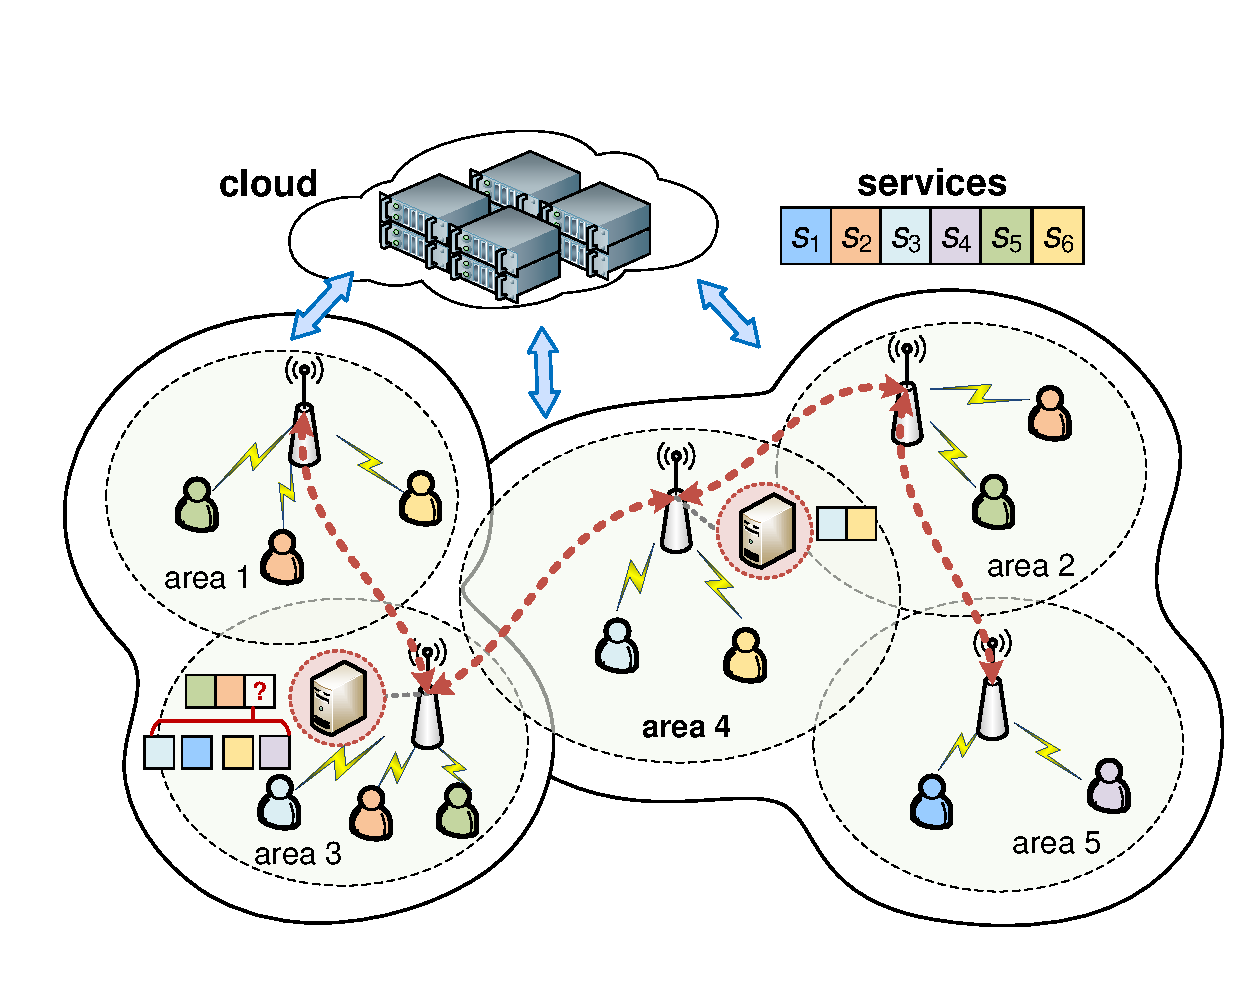
\includegraphics[width=1.0\columnwidth]{figure1_user_selected_no_outer_border.pdf}
    \caption{MEC system model and service-provisioning scenario.}
    \label{fig1}
\end{figure}

\subsection{Motivation and Challenges}

Server deployment and service provisioning have a significant impact on the profit of mobile network operators. Figure~\ref{fig1} illustrates a scenario with five base stations. The solid black contours partition the topology into interconnected service regions, the black dashed circles denote the coverage areas of individual base stations, and the red dotted circles identify base stations equipped with edge servers. The blue bidirectional arrows represent cloud--edge communication, while the red dashed arrows indicate inter-region request forwarding. Distinct colors represent service types $s_1$--$s_6$, and each user color indicates the corresponding requested service. The service blocks beside an edge server show its instantiated services; the question-mark slot in Area~3 denotes a provisioning decision under limited server capacity.
Each service replica serves a user request and generates income. Because an edge server can host only a subset of the service catalog, a request without a local replica is forwarded to another server that provides the requested service, incurring additional transmission cost. For example, the server in Area~4 provisions services $s_3$ and $s_6$; requests for the other service types require inter-area forwarding. This setting gives rise to the following two challenges:


(i) Determining the optimal number and location of edge servers to maximize user coverage across diverse regions while minimizing the overall deployment cost for mobile network operators remains a critical challenge. As illustrated in Figure~\ref{fig1}, deploying only a single server results in the lowest deployment cost but fails to cover all users, while deploying one server in each of the five areas incurs prohibitively high expenses. In this paper, we consider the spatial distribution of user densities and strategically deploy servers only in areas 3 and 4. Leveraging the connectivity among base stations, this deployment strategy provides service to the maximum number of users at a moderate total cost. Through this approach, we achieve a balance between server deployment cost and transmission cost.\par
%图片修改一下，服务器放area3，然后在空余的那个槽位底下以两个带颜色的服务和问号指向该空白槽位，示意出于不同的角度考虑可以有多种部署策略。

(ii) Designing an effective service provisioning strategy under constrained server capacity while jointly optimizing provisioning cost and users' delay remains a significant challenge. For example, the server in Area~3 can host three service instances. Two slots are occupied by the illustrated service replicas, while the remaining slot must be assigned from the candidate services shown below the server. Since this choice affects forwarding distance, transmission cost, and service-delivery latency, the provisioning decision considers request frequency and service provisioning cost. Therefore, an appropriate combination of server deployment and service provisioning decisions is crucial for maximizing the profit of mobile network operators.

% (i). How to determine the number and deployment locations of servers that can be able to serve as many users as possible in various areas considering the cost of mobile network operators. %在图1中，只放置一台服务器成本消耗最低，但无法覆盖全部用户，而在五个区域全部放置服务器则会大量开销。本文结合用户区域密度的分布，将服务器放置在area3与area4，借助基站彼此间的连通性，以适中的成本为尽可能多的用户提供服务。通过该种放置策略，实现放置成本与通讯成本间的平衡。
% %%%%图片修改一下，服务器放area3，然后在空余的那个槽位底下以两个带颜色的服务和问号指向该空白槽位，示意出于不同的角度考虑可以有多种部署策略。
% (ii). How to determine service placement strategies within limited server capacity to increase the profit of mobile network operators.%以area4的服务器为例，它具有三个服务容量，无法满足所有需要提供服务的用户。其上面已经放置了$s_{3}$ 和 $s_{6}$号服务，但需要结合用户请求频率，服务部署成本以及可提供的潜在收益来确定最后一个容量部署哪种服务。Once the service placement phase within $area_{3}$ is completed, servers begin to handle service requests. The server's deployment phase affects transmission cost, which in turn impacts the speed of service delivery, influencing user satisfaction. Satisfied users are more likely to use the service again, increasing mobile network operators' profit. Therefore, it has become extremely important to use the right server deployment and service provisioning strategy to increase mobile network operators' profit.

\subsection{Contributions and Paper Organization}
In this paper, we investigate the problem of server deployment and service provisioning in a multi-user scenario, aiming to jointly optimize the cost and user access latency under multiple constraints such as distance thresholds, resource limitations, and connectivity requirements. Our research contributions are summarized as follows:
\begin{itemize}
  \item We develop a joint server-service optimization model to address the challenges of server deployment and service provisioning in multi-user scenarios. To better tackle this problem, we use a decomposition that separates it into two sequential stages. The first stage, server deployment, focuses on servers, determining where edge servers should be deployed. The second stage, service provisioning, involves deciding the provisioning locations of services across the selected servers. 
  \item We formalize the first stage server deployment as a $k$-median problem and introduce a Coverage-based Local Search (CLS) strategy to determine optimal server locations. Building upon the deployment of servers, the second stage addresses service provisioning through an enhanced strategy featuring improved initial population generation with high-quality solutions. This constitutes our proposed Pareto-oriented Service Provisioning (PSP) approach, achieving joint optimization of provisioning cost and service latency.
  \item We conducted extensive experiments to compare our strategy with several baselines based on a real-world base station dataset provided by Beijing Telecom. The results are shown from different perspectives to provide conclusions. Extensive experiments demonstrate the superior performance of the proposed algorithms.
\end{itemize}

The remainder of this paper is organized as follows. In Section II, we review related research. In Section III, we model the problem. In Section IV, we propose the server deployment and service provisioning algorithms. In Section V, we present the comparative experimental results. Finally, in Section VI, we conclude the paper.

\section{RELATED WORK}
%这部分是论文的相关工作，第一段简要介绍，当前的研究多数关注单目标优化，少有对成本、延迟进行联合优化，因此本文选择对多目标优化方向进行研究。
%service provisioning 不用placement；server没问题 在每段最后自己总结一下，说明一下共性问题
%目前关于移动边缘计算的研究中，涉及到服务器和服务的部署策略多为仅考虑部署成本或用户延迟其中单独一个方面，少有对两方面进行联合优化的研究，导致运营商利益和用户需求往往不能同时满足。因此，本文针对上述提到的当前边缘计算应用背景下存在的相关问题，设计了面向成本延迟联合优化的边缘服务器与服务部署策略。
% \subsection{server deployment}
%边缘服务器放置问题的解决方法多样，Wang等[4]采用混合整数规划和理论证明寻找边缘服务器放置的最优解，用于降低访问延迟，优化负载均衡。Li等[7]设计了一种基于粒子群优化的节能边缘服务器布局算法来寻找服务器放置布局问题的最优解。Xu等[8]设计了一种在5G网络中通过构建一棵决策树并结合非支配排序遗传算法II（ Non-dominated Sorting Genetic Algorithm II，NSGA-II）获取均衡的边缘服务器布局策略的负载感知边缘服务器部署方法。Jiang等[9]提出了两种基于深度强化学习的算法实现智能动态调整服务器布局。Kasi S K等[10]使用遗传算法快速搜索大型解空间以找到最小化成本函数的边缘放置策略。Wu等[11]提出了三种贪婪启发式算法来解决服务器布局问题。Shen等[12]提出了一种动态 ES 部署方法 (DEP)来进行服务器的部署。然而，上述服务器放置策略多数仅关注能耗和负载均衡方面，少有结合用户分布这一特性进行服务器放置，使得决策在用户向的考虑有所欠缺。
% \subsection{service provision}
%在解决有关服务部署的问题上，Qian等[16]提出了一种隐私感知的服务部署方案和一种集中式贪婪算法与分布式联邦学习相结合的混合服务放置算法，既能保护用户的隐私，又能通过移动边缘云满足用户的服务需求。Yu等[13]研究了MEC中的协同服务部署问题，提出了一种基于匹配理论的高效分散算法来优化基站的服务放置和基站-用户设备关联决策。Ma等[15]研究了在长期成本预算约束下移动边缘服务布局的性能优化问题，通过一种基于帧设计的T槽预测服务布局算法进行性能提升。Ouyang等[16]研究了长期成本预算约束下的移动边缘服务性能优化问题，应用Lyapunov optimization方法将长期优化问题分解为一系列实时优化问题。此外，他还指出现有研究侧重于研究系统级服务放置问题，鲜有关注个性化服务功能。因此，提出了一种新颖的自适应用户管理服务放置机制，联合优化用户的感知延迟和服务迁移成本，帮助实现自适应服务放置决策[17]。Zhang等[18]提出了一个基于控制论和博弈论模型的动态框架来解决服务部署问题。Skarlat O等[19]提出了一个雾计算概念框架，使用一种遗传算法作为解决问题的方案。Wang等[20]提出了一种具有多项式时间复杂度的在线近似算法，用于在实例到达时实时找到服务部署位置。Wang和Jiao等[21]提出了一种名为 ITEM 的迭代算法来部署协作式边缘服务。然而，这些策略大多面向同质任务请求，或仅面向满足用户请求，未充分考虑服务对象任务请求之间的差异性，导致资源分配低效，忽视了从服务提供商角度出发的利润需求。
%本论文针对上述提到的当前边缘计算应用背景下存在的相关问题，设计了面向成本延迟联合优化的边缘服务器与服务部署策略。该方法会在降低部署成本的同时降低用户时延，高效地实现边缘节点与服务部署，提升网络性能、优化资源分配。
In recent years, a substantial body of research in mobile edge computing (MEC) has focused on either reducing deployment cost or minimizing user latency. However, few studies address the joint optimization of both objectives. As a result, it is often difficult to simultaneously satisfy both operator profitability and user quality of service. To bridge this gap, this paper investigates the cost-latency joint optimization of edge server deployment and service provision.

\subsection{Server Deployment}
Various methods have been proposed to solve the edge server deployment problem. Wang et al.~\cite{b1} used mixed-integer programming with theoretical guarantees to obtain optimal placements aimed at minimizing access latency and balancing system loads. Li et al.~\cite{b2} developed a particle swarm optimization-based layout algorithm for energy-efficient server deployment. Xu et al.~\cite{b3} proposed a load-aware deployment strategy that leverages decision trees and NSGA-II to construct balanced layouts. Jiang et al.~\cite{b4} introduced two deep reinforcement learning-based algorithms for dynamic server placement. Kasi et al.~\cite{b5} utilized genetic algorithms to explore large solution spaces for cost-minimizing deployment. Wu et al.~\cite{b6} proposed three greedy heuristics, and Shen et al.~\cite{b7} designed a dynamic deployment method. Ling et al.~\cite{b8} formulated the edge server placement problem as a constrained optimization problem and applied the Particle Swarm Optimization (PSO) algorithm to optimize network latency and energy consumption jointly. Luo et al.~\cite{b9} proposed an edge server placement algorithm named DQN-ESPA, which leverages Deep Q-Networks and reinforcement learning to achieve optimal placement without relying on prior deployment experience. Zeng et al.~\cite{b10} developed a global optimization method based on simulated annealing and a greedy heuristic to satisfy capacity constraints of edge servers while minimizing the number of simultaneously active edge servers, thus enabling efficient and cost-effective deployment. Guo et al.~\cite{b11} proposed an approximate method using k-means and mixed-integer quadratic programming to balance the workload among edge clouds. Xu et al. ~\cite{b12} studied the joint deployment and allocation of virtual network functions, aiming to achieve a balance between cost and QoS. Cui et al.~\cite{b13} modeled this joint user coverage and network robustness oriented k-edge server placement problem and showed that finding the optimal solution to the problem is NP-hard. However, most of these server deployment strategies focus primarily on energy efficiency and load balancing, with limited consideration of user distribution. This lack of user-centric design leads to placement decisions that may overlook demand-side characteristics, potentially reducing the overall effectiveness of deployment strategies.

\subsection{Service Provision}
For service provision, Qian et al.~\cite{b14} proposed a privacy-aware provisioning framework combining a centralized greedy algorithm with distributed federated learning, enabling both privacy protection and efficient service delivery through mobile edge clouds. Yu et al.~\cite{b15} explored collaborative service provision and proposed a distributed algorithm based on matching theory to jointly optimize service placement and user association. Ma et al.~\cite{b16} investigated long-term cost-constrained service layout and introduced a T-slot frame-based predictive provisioning algorithm to enhance system performance. Ouyang et al.~\cite{b17} applied Lyapunov optimization to transform long-term constraints into real-time decision problems. Furthermore, they proposed an adaptive user-aware management mechanism that jointly optimizes perceived latency and service migration costs~\cite{b18}. Zhang et al.~\cite{b19} built a dynamic framework using control theory and game-theoretic modeling. Skarlat et al.~\cite{b20} proposed a fog computing framework utilizing genetic algorithms, while Wang et al.~\cite{b21} developed an online approximation algorithm with polynomial complexity for real-time service provisioning. Wang and Jiao~\cite{b22} presented an iterative algorithm for collaborative edge service deployment. Cabrera C et al.~\cite{b23} proposed a mobility-aware, priority-driven, ACO-based service deployment model that aims to minimize latency for critical applications by predicting the mobility paths of users. However, this model sacrifices load balancing among network servers. Yang et al.~\cite{b24} leveraged user mobility patterns and service access behaviors to predict the future distribution of service requests, and dynamically adjusted service placement and load scheduling based on these predictions to reduce latency caused by accessing remote cloud servers. Chen et al.~\cite{b25} investigated the problem of edge service deployment for application service providers under limited budget constraints, and they proposed a spatio-temporal edge service placement algorithm to enhance the performance of edge computing. Han et al. ~\cite{b26} addressed energy-saving and flexible service layout in mobile edge cloud networks supporting cell scaling. Sami et al.~\cite{b27} proposed a deep reinforcement learning solution for fast and proactive service updates to meet user needs. %Li et al.~\cite{b28} proposed a collaborative placement and scheduling framework for joint optimization design. 
However, most of these strategies assume homogeneous service requests or focus solely on satisfying user demands, without adequately accounting for the heterogeneity of task requirements. This results in inefficient resource allocation and ignores the profitability concerns of service providers.


Optimization and learning methods also address complementary MEC resource-management objectives. Feng et al.~\cite{b33} jointly optimized latency-aware service deployment and peer offloading over multiple timescales. Kato et al.~\cite{b34} applied breakout local search to transmission- and processing-aware task offloading in a multi-tier cloud environment. Jing et al.~\cite{b35} studied long-term max--min fairness for task splitting and resource allocation in integrated multi-RAT/MEC networks, while Jing et al.~\cite{b36} used online mini-batch learning for dynamic energy-cost conservation in distributed edge clouds. These studies address dynamic offloading, fairness, or energy management; the present work focuses on interpretable server planning and capacity-constrained multi-objective service provisioning under a common cost--latency model.


To address the limitations outlined above, we propose a joint optimization framework for edge server deployment and service provision. The proposed strategy aims to simultaneously reduce deployment costs and user latency, thereby enhancing network performance and resource efficiency in MEC environments.

\section{Model and Problem Formulation}
In this paper, we focus on an optimization problem involving server deployment and service provisioning in a mobile edge computing environment. To jointly minimize latency and cost while satisfying constraints such as storage capacity and transmission bandwidth, we construct a comprehensive system model. Our objective is to optimize resource allocation and service provisioning strategies, considering constraints on resources and geographical distance. 
\subsection{The MEC Environment}
In this paper, we consider a hierarchical network architecture comprising the cloud data center, edge servers, and mobile end users, as illustrated in Figure~\ref{fig1}. The cloud layer serves as a centralized resource pool that hosts all services required by user requests. We use $\mathcal{S} = \{s_w\}$ to denote the set of services that are requested by users. For each service $s_w$, the consumption of storage resources is indicated by $v_{w}$, and the required computing resource is denoted by $\varsigma_{w}$. At the edge layer, each edge server is assumed to be co-located with a base station and is responsible for provisioning services to support user access and process tasks near the user side. The set of base stations is denoted by $\mathcal{B} = \{b_k\}$, where $b_k$ represents the $k$-th base station. Mobile network operators deploy edge servers according to the locations of base stations. The set of edge servers is denoted by $\mathcal{M} = \{m_j\}$, where $m_j$ represents the $j$-th server. Let $V_j$ denote the storage capacity of edge server $m_j$, indicating the maximum amount of storage resources available for service deployment. The set of services deployed on $m_j$ is represented by $S_j$. At the user layer, the set of mobile users is denoted by $\mathcal{U} = \{u_i\}$, where $u_i$ represents the $i$-th user. Each user generates a service request $u_{iw}$, and multiple users may request the same type of service, which is represented by the set $\mathcal{U}_{w}=\{u_{iw}\}$. Key notations are summarized in Table~\ref{table:variables_extended} for clarity. 

\subsection{Cost Model}
Mobile network operators are responsible for deploying edge servers and provisioning services to accommodate user requests, resulting in costs associated with server deployment, service provisioning, and data transmission. 
\subsubsection{Server Deployment Cost} 

The server deployment cost refers to the inherent cost incurred when deploying an edge server co-located with a base station. We assume that the servers are heterogeneous and that the deployment cost of server $m_j$ is denoted by $p_j$. Let $y_{jk}$ be a binary server-deployment variable, where $y_{jk}=1$ if edge server $m_j$ is deployed at base station $b_k$, and $y_{jk}=0$ otherwise. Accordingly, the deployment cost of server $m_j$ is $C_{d}(m_j)=y_{jk}p_j$.

%Accordingly, the total server deployment cost is defined as the sum of the costs of all deployed servers, where $C_{d} = \sum_{j\in \textbf{M}} p_j$.

\subsubsection{Service Provisioning Cost} 

The service provisioning cost is represented by the set $\mathcal{SC}=\{sc_w\}$, where $sc_w$ denotes the provisioning cost of service $s_w$. Let $z_{jw}$ be a binary service-provisioning variable, where $z_{jw}=1$ if an instance of $s_w$ is provisioned on edge server $m_j$, and $z_{jw}=0$ otherwise. Furthermore, let $a_{ijw}$ be a binary association variable, where $a_{ijw}=1$ if user $u_i$ is served by service $s_w$ on server $m_j$, and $a_{ijw}=0$ otherwise. The total provisioning cost of server $m_j$ is $C_p(m_j)=\sum_{s_w\in\mathcal{S}}z_{jw}sc_w$.


\subsubsection{Transmission Cost}
The transmission cost is produced by the physical distance between users and their assigned servers during network communications. Each user is associated with a server that provides the requested service, and a per-unit distance transmission cost coefficient is defined accordingly. Specifically, we assume that if a user is located within the optimal service coverage radius of its assigned server and the server can provide the requested service, the per-unit transmission cost coefficient is set to be $0$, which indicates no transmission cost. If the user is located outside the optimal coverage area but the assigned server can still provide the requested service, the coefficient is set to the base value. If the assigned server cannot provide the requested service, the coefficient increases proportionally with the number of intermediate servers traversed during service routing. Finally, if no available service instance can be found after searching the entire area, the coefficient reaches its maximum value, which is defined as $k$ times of the base value, where $k$ corresponds to the total number of servers. Consequently, the transmission cost is modeled as the product of the physical distance between users and edge servers and the corresponding per-unit distance transmission cost coefficient, which is defined as $C_{t}(m_j) = \sum_{i \in U} \alpha\cdot \beta_{iw}\cdot\tau_{(u_i \rightarrow m_j)}$. Here, we use $\alpha$ to denote the unit price of communication bandwidth, $\beta_{iw}$ represents the number of hops between the location of user $u_i$ and the edge server providing service $s_w$, and $\tau(u_i \rightarrow m_j)$ denotes the physical distance between user $u_i$ and $m_j$.

Therefore, the total cost for services provided by server $m_j$ is defined as follows: 
\begin{equation}
\mathbb{C}(m_j) = C_{d}(m_j) + C_{p}(m_j) + C_{t}(m_j).
	 \label{eq1}
\end{equation}

% The cost for services provided by $e_j$ is defined as follows:
% \begin{equation}
	% C_{e_j} = C_{e_j}^{alloc} + C^{trans} + C_{e_j}^{comp}.
	% \label{eq1}
	% \end{equation}
% Intuitively, the profit of $e_j$ can be expressed as:
% \begin{equation}
	% O_{e_j} = I_{e_j} - C_{e_j}.
	% \label{eq2}
	% \end{equation}
% Our overall objective is to maximize the profit of all servers.

%在本文中，用户集合记作 $U = {u_i}$，其中 $u_i$ 表示第 $i$ 个用户；服务器集合记作 $M = {m_j}$，其中 $m_j$ 表示第 $j$ 个服务器；服务集合记作 $S = {s_w}$，其中 $s_w$ 表示第 $w$ 个服务；基站集合记作 $B = {b_k}$，其中 $b_k$ 表示第 $k$ 个基站；服务部署成本集合记作 $SC = {sc_w}$，其中 $sc_w$ 表示第 $w$ 个服务的部署成本。
%我们设置一个总开销上限 $C_{max}$，表示服务器放置部分允许的总成本上限，对应的最多可放置服务器节点数为 $N_1$。考虑到用户密度因素的影响，本文引入用户密度阈值 $\sigma_{min}$，并为每个服务器设定一个最优服务覆盖半径 $r$，则所有满足该密度阈值条件的基站数记为 $N_2$。
%二进制变量 $x_{jw}$ 表示服务 $s_w$ 是否部署在服务器 $m_j$ 上，若部署则 $x_{jw} = 1$；其部署成本为 $sc_w$。变量 $x_{ijw}$ 表示用户 $u_i$ 是否使用部署在服务器 $m_j$ 上的服务 $s_w$，若使用则 $x_{ijw} = 1$，否则为 0。每台边缘服务器 $m_j$ 的存储能力为 $V_j$，计算能力为 $\mu_j$。
% \begin{table}[!t]
% 	\centering
% 	\caption{SUMMARY OF SYMBOLS IN THE SYSTEM MODEL}
% 	\label{table:variables_extended}
% 	\begin{tabular}{|c|p{6cm}|}
% 		\hline
% 		\textbf{Symbol} & \textbf{Definition} \\
% 		\hline
% 		$\textbf{U}$ & Set of users, $U = \{u_i\}$ \\ \hline
% 		$\textbf{M}$ & Set of servers, $M = \{m_j\}$ \\ \hline
% 		$\textbf{S}$ & Set of services, $S = \{s_w\}$ \\ \hline
% 		$\textbf{B}$ & Set of base stations, $B = \{b_k\}$ \\ \hline
% 		$\textbf{SC}$ & Set of service deployment costs, $SC = \{sc_w\}$ \\ \hline
% 		$p_j$ & Deployment cost of server $m_j$ \\ \hline
% 		$x_{ij}$ & Indicator whether user $u_i$ is served by $m_j$.\\ \hline
%             $x_{jk}$ & Indicator whether server $m_j$ is deployed at base station $b_k$.\\ \hline
% 		$x_{ijw}$ & Indicator whether user $u_i$ is served by $s_w$ on $m_j$. \\ \hline
% 		$x_{jw}$ & Indicator whether server $m_j$ deploys service $s_w$ (1 if deployed) \\ \hline
% 		$C_{max}$ & Maximum allowed total server deployment cost \\ \hline
% 		$\mathcal{K}^c$ & Maximum number of deployable server nodes under $C_{max}$ \\ \hline
% 		$r$ & Optimal service coverage radius of each base station \\ \hline
% 		$\sigma_{min}$ & Minimum required user density \\ \hline
% 		$\mathcal{K}^r$ & Number of base stations whose local user density exceeds the threshold $\sigma_{min}$ \\ \hline
% 		$k$ & Number of servers actually deployed \\ \hline
% 		$\alpha$ & Unit price of communication bandwidth \\ \hline
%             $\beta_{iw}$ & Number of hops between the location of user $u_i$ and the edge server providing service $s_w$ \\ \hline
% 		$\tau(u_i \rightarrow m_j)$ & Distance between user $u_i$ and server $m_j$ \\ \hline
% 		$V_j$ & Service capacity of server $m_j$ \\ \hline
% 		$R^{\textbf{c}}_{iw}$ & Required computation resource for user $u_i$ to request service $s_w$ \\ \hline
%             $R^{\textbf{t}}_{iw}$ & Data volume transmitted by user $u_i$ \\ \hline
% 		$\mu_j$ & Computing capacity of server $m_j$ \\ \hline
% 		$r_{ij}$ & Maximum transmission rate from $u_i$ to $m_j$ \\ \hline
% 		$\widetilde{D_i}$ & Maximum tolerable transmission delay of $u_i$ \\ \hline
		
% 	\end{tabular}
% \end{table}

\begin{table}[!t]
\centering
\caption{SUMMARY OF SYMBOLS IN THE SYSTEM MODEL}
\label{table:variables_extended}
\begin{tabular}{|>{\centering\arraybackslash}m{2cm}|>{\raggedright\arraybackslash}m{6cm}|}
    \hline
    \textbf{Symbol} & \textbf{Definition} \\
    \hline
    $\mathcal{U}$ & Set of users, $U = \{u_i\}$ \\ \hline
    $\mathcal{M}$ & Set of servers, $M = \{m_j\}$ \\ \hline
    $\mathcal{S}$ & Set of services, $S = \{s_w\}$ \\ \hline
    $\mathcal{B}$ & Set of base stations, $B = \{b_k\}$ \\ \hline
    $\mathcal{SC}$ & Set of service deployment costs, $SC = \{sc_w\}$ \\ \hline
    $p_j$ & Deployment cost of server $m_j$ \\ \hline
    $a_{ij}$ & Indicator whether user $u_i$ is served by $m_j$.\\ \hline
    \multirow{2}{*}{$y_{jk}$} & Indicator whether server $m_j$ is deployed \\ 
    & at base station $b_k$.\\ \hline
    $a_{ijw}$ & Indicator whether user $u_i$ is served by $s_w$ on $m_j$. \\ \hline
    $z_{jw}$ & Indicator whether server $m_j$ provisions service $s_w$. \\ \hline
    $C_{max}$ & Maximum allowed total server deployment cost \\ \hline
    $\mathcal{K}^c$ & Maximum number of deployable server nodes under $C_{max}$ \\ \hline
    % $r$ & Optimal service coverage radius of each base station \\ \hline
    $\sigma_{min}$ & Minimum required user density \\ \hline
   $\mathcal{K}^r$ & Number of base stations with local user density exceeds $\sigma_{min}$ \\ \hline
    $k$ & Number of servers actually deployed \\ \hline
    $\alpha$ & Unit price of communication bandwidth \\ \hline
    $\beta_{iw}$ & Number of hops between user $u_i$ and server $m_j$ providing $s_w$. \\ \hline
    $\tau(u_i \rightarrow m_j)$ & Distance between user $u_i$ and server $m_j$ \\ \hline
    $V_j$ & Service capacity of server $m_j$ \\ \hline
    \multirow{2}{*}{$R^{\textbf{c}}_{iw}$} & Required computation resource for \\ 
    & user $u_i$ requesting $s_w$ \\ \hline
    $R^{\textbf{t}}_{iw}$ & Data volume transmitted by user $u_i$ \\ \hline
    $\mu_j$ & Computing capacity of server $m_j$ \\ \hline
    $r_{ij}$ & Maximum transmission rate from $u_i$ to $m_j$ \\ \hline
    $\widetilde{D_i}$ & Maximum tolerable transmission delay of $u_i$ \\ \hline
\end{tabular}
\end{table}

\subsection{Latency Model}

In this system, user latency occurs during both computation and communication. We define $D_{p}(m_j)$ as the computational latency associated with user requests processed by edge server $m_j$. This latency depends on the resource requirements of the requested services and the computing capabilities of the servers, and is given by $D_{p}(m_j)=\sum_{i\in\mathcal{U}}a_{ijw}R^{\textbf{c}}_{iw}/\mu_j$, where $\mu_j$ denotes the computing capacity of edge server $m_j$, $R^{\textbf{c}}_{iw}$ represents the computational resource demand of service $s_w$ requested by user $u_i$, and $a_{ijw}$ indicates whether $u_i$ is served by $s_w$ on $m_j$.

%这里假设的是并行处理的，总的计算资源请求不能超过总core数


In addition, communication latency refers to data transmission between users and edge servers when a requested service is provisioned outside the user's region. It is influenced by the propagation and transmission times of the network, where the propagation delay depends on the distance $\tau(u_i\rightarrow m_j)$ between user $u_i$ and edge server $m_j$ hosting service $s_w$. We define the maximum transmission rate as $r_{ij}=B_{ij}\log_2\!\left(1+\gamma g_{ij}/\mathcal{N}\right)$~\cite{b28,b31,b32}, where $B_{ij}$ denotes the channel bandwidth, $\gamma$ is the transmission power of the user device, $\mathcal{N}$ is the noise power, and $g_{ij}$ is the channel gain between $u_i$ and $m_j$. The channel gain is modeled as $g_{ij}=127+30\log\!\left(\tau(u_i\rightarrow m_j)\right)$. For each user, the transmitted data volume is denoted by $R^{\textbf{t}}_{iw}$. When a requested service is unavailable at the nearest server, the request is forwarded through intermediate servers; $\beta_{iw}$ captures the resulting per-hop communication delay. Consequently, the communication latency is $D_c(m_j)=\sum_{i\in\mathcal{U}}a_{ijw}(R^{\textbf{t}}_{iw}/r_{ij})\beta_{iw}$.

Therefore, the total latency for users provided by server $m_j$ is defined as follows: 
% \cdot g_{ij}}/{\mathcal{N}} \right)$~\cite{lu1}, where $B_{ij}$ denotes 
\begin{equation}
	\mathbb{D}(m_j) = D_{p}(m_j) + D_{c}(m_j).
	\label{eq2}
\end{equation}
% The cost for services provided by $e_j$ is defined as follows:
% \begin{equation}
% C_{e_j} = C_{e_j}^{alloc} + C^{trans} + C_{e_j}^{comp}.
% \label{eq1}
% \end{equation}
% Intuitively, the profit of $e_j$ can be expressed as:
% \begin{equation}
% O_{e_j} = I_{e_j} - C_{e_j}.
% \label{eq2}
% \end{equation}
% Our overall objective is to maximize the profit of all servers.

\subsection{Problem Formulation}
On the basis of the models above, our objective is to design an efficient strategy that jointly minimizes the total cost and latency, while considering user mobility under the system constraints. Thus, the optimization objective is formulated as follows: 
\begin{align}
	&\textbf{P}_1:\text{minimize} \quad \sum_{m_j\in \textbf{M}}\textbf{Q}(\mathbb{D}(m_j), \mathbb{C}(m_j))\label{eq3}\\
&\text{s.t.} \quad \sum_{m_j\in \textbf{M}} C_{d}(m_j) \leq C_{\max},\label{eq4}\\
% & 0 \leq \beta_{iw} \leq k \label{const:ab_range} \\
& \sum_{w \in \mathcal{S}} z_{jw}v_w \leq V_j, \quad \sum_{w \in S_j} z_{jw}\varsigma_w \leq \mu_j, \,\label{eq5} \\
& a_{ijw}\left({R^{\textbf{c}}_{iw}}/{\mu_j} + ({R^{\textbf{t}}_{iw}}/{r_{ij}})\beta_{iw}\right) \leq \widetilde{D_i}, \quad \forall i \in \mathcal{U}, \label{eq6} \\
& y_{jk}, z_{jw}, a_{ijw} \in \{0,1\}, \quad \forall i \in \mathcal{U}, \, \forall j \in \mathcal{M}.\label{eq7}
\end{align}  

$\textbf{P}_1$ is the objective function, and Eqs.~(\ref{eq4})--(\ref{eq7}) specify its constraints. Equation~(\ref{eq4}) limits total server-deployment cost to budget $C_{\max}$. Equation~(\ref{eq5}) enforces the storage and computing capacities of each edge server. Equation~(\ref{eq6}) provides latency-oriented QoS by requiring the end-to-end latency of a served request to remain below the user's tolerable bound $\widetilde{D_i}$. For reliability-critical applications, latency compliance can be complemented by packet-loss, link-availability, and service-interruption constraints, preventing a low-latency solution from being selected when service continuity is insufficient. Equation~(\ref{eq7}) defines the server-deployment variable $y_{jk}$, service-provisioning variable $z_{jw}$, and user-service association variable $a_{ijw}$.

%constraints -- 下面前两段为Lu已经列好的英文，Xu的解释将紧接着用中文先行给出
%%%%限制条件续，接着上文的N_c,N_r，目前我仍然沿用k作为二者其中的较小者记为放置server的数量，如认为无必要可删去%%%%%%
%我们将 $k$ 定义为 $N^c$ 与 $N_r$ 之间的较小值，记它为需要放置的服务器的数量。P1 is the objective function. Equations~(4) to (8) are the constraints。其中，公式（4）为放置成本约束，要求部署服务器的总成本不能超过上限 $C_{\max}$。
%公式（5）为用户请求的服务在中转时的跳数的取值最低为 $0$，即不进行中转；最高为所有放置的服务器数量 $k$，即遍寻全部服务器。
%公式（6）说明物理资源限制，边缘服务器 $m_j$ 上部署的服务所需存储资源总和 $\sum_{w \in S} x_{jw}$ 不超过其存储能力 $V_j$，边缘服务器 $m_j$ 上部署的服务所需计算资源总和 $\sum \mu_{s_w}^j$ 不超过其计算能力 $\mu_j$。公式（7）表示计算得出用户延迟必须小于等于用户可容忍的最大延迟 $D_{\max}$。公式（8）分别表示用户 $u_i$ 是否选择服务器 $m_j$，基站 $b_k$ 是否部署服务器 $m_j$，服务 $s_w$ 是否部署在服务器 $m_j$ 上，以及用户 $u_i$ 是否使用服务器 $m_j$ 上的服务 $s_w$。为了求解该问题，我们将问题拆分为两阶段来对其进行解耦。
To solve this problem, we use a decomposition that separates it into two sequential stages. The first stage focuses on servers, determining where edge servers should be deployed. The second stage addresses providing services, i.e., deciding the provisioning locations of services across the selected servers. 


The decomposition follows the operational hierarchy of MEC planning. Server deployment is a long-term infrastructure decision governed by budget, coverage, and geographic demand, whereas service instances are provisioned after the physical server locations are known. Stage~1 therefore resolves the spatial variables that determine deployment and transmission costs, and Stage~2 optimizes service instances and user associations on the selected infrastructure. Passing the selected locations, user assignments, and Stage-I cost to Stage~2 preserves the cost--latency dependence while substantially reducing the decision space of the service-provisioning search.


In the first stage (server deployment), we isolate the cost terms $C_{d}(m_j)$ and $C_{t}(m_j)$ from the original problem $\textbf{P}_1$ and consider them as the primary objective for this stage, since both are directly influenced by the locations of the deployed edge servers. The trade-off in the first stage is that reducing the deployment cost $C_{d}(m_j)$ may lead to increased transmission cost $C_{t}(m_j)$, and vice versa. Therefore, our objective is to balance these two costs by solving the following optimization problem:
\begin{align}
&\textbf{P}_2:\quad \text{minimize} \quad \sum_{m_j\in \textbf{M}}C_{d}(m_j) + C_{t}(m_j) \label{eq:p2_obj} \\
&\text{s.t.} \quad (\ref{eq4}), (\ref{eq7}) \label{eq:p2_constraints}
\end{align}
According to the above formulation, this stage aims to determine the server deployment strategy, including both the number and locations of edge servers to be deployed. The problem is NP-hard and can be reduced to the classical set cover problem~\cite{b29,b30}. 
%从下面开始为Stage I的解释By Xu（这段的开始使用了论文原文，意在阐述放置成本和传输成本成反比的关系，因为放置成本的减少势必会带来传输成本的增加，反之亦然）
%In stage I, we isolate the portion $C_{depl} + C^{trans}$ from $\textbf{P}_1$ for separate analysis, considering it as the objective of stage I. This phase presents a balancing act, as reducing $C_{depl}$ results in an increase of $C^{trans}$ and vice versa. 因此在stage 1中本文计划在这两项成本间取得平衡。定义stage 1的目标函数为；minimize C_depl+C_tran;s.t.(1)-(2);(这个的latex在上面)该函数主要与服务器放置有关，因此我们会在该阶段确定服务器放置策略，包括待放置的个数和位置。该问题是NP-hard problem,can be reduced to set cover problem \cite(set).
% \subsection{Stage II-Service Provisioning}

In the second stage (service provisioning), we address the remaining portion of the original problem $\textbf{P}_1$. The resulting cost value $\widetilde{\mathbb{C}}$ from the first stage is treated as a fixed input in the second stage, which focuses on the joint optimization of the remaining provisioning cost $C_{p}(m_j)$ and service latency $\mathbb{D}(m_j)$. The objective function is defined as follows:
\begin{align}
&\textbf{P}_3:\quad \text{minimize} \quad \sum_{m_j \in \textbf{M}} \textbf{Q}\big(\mathbb{D}(m_j), C_{p}(m_j), \widetilde{\mathbb{C}}\big) \label{eq:p3_obj} \\
&\text{s.t.} \quad (\ref{eq5})\sim (\ref{eq7}) \label{eq:p3_constraints}
\end{align}
Therefore, we are concerned with the cost of service provisioning and user-perceived latency by designing a strategy that jointly optimizes the remaining provisioning cost and latency in a fixed server configuration.  
%从下面开始为Stage II的解释By Xu（这段的开始使用了论文原文，意在阐述我们接下来将解决剩余问题）
%In stage II, we will address the remaining portion of $\textbf{P}_1$. In stage I, 我们已经为$C_{depl}$ 和 $C^{trans}$取得了一定的平衡。在该阶段，我们将stage 1得出的该值作为一个定值参与本阶段的联合优化，则优化目标重新记为\textbf{Q}'\big,成本函数重新记为\mathbb{C}'(m_j)\big，\mathbb{D}(m_j)保持不变。这样，该阶段的目标函数主要与服务部署成本和用户延迟有关，我们在该阶段设计服务部署策略，以实现对剩余成本和延迟的联合优化。

\begin{figure*}[!t]
 \centering
    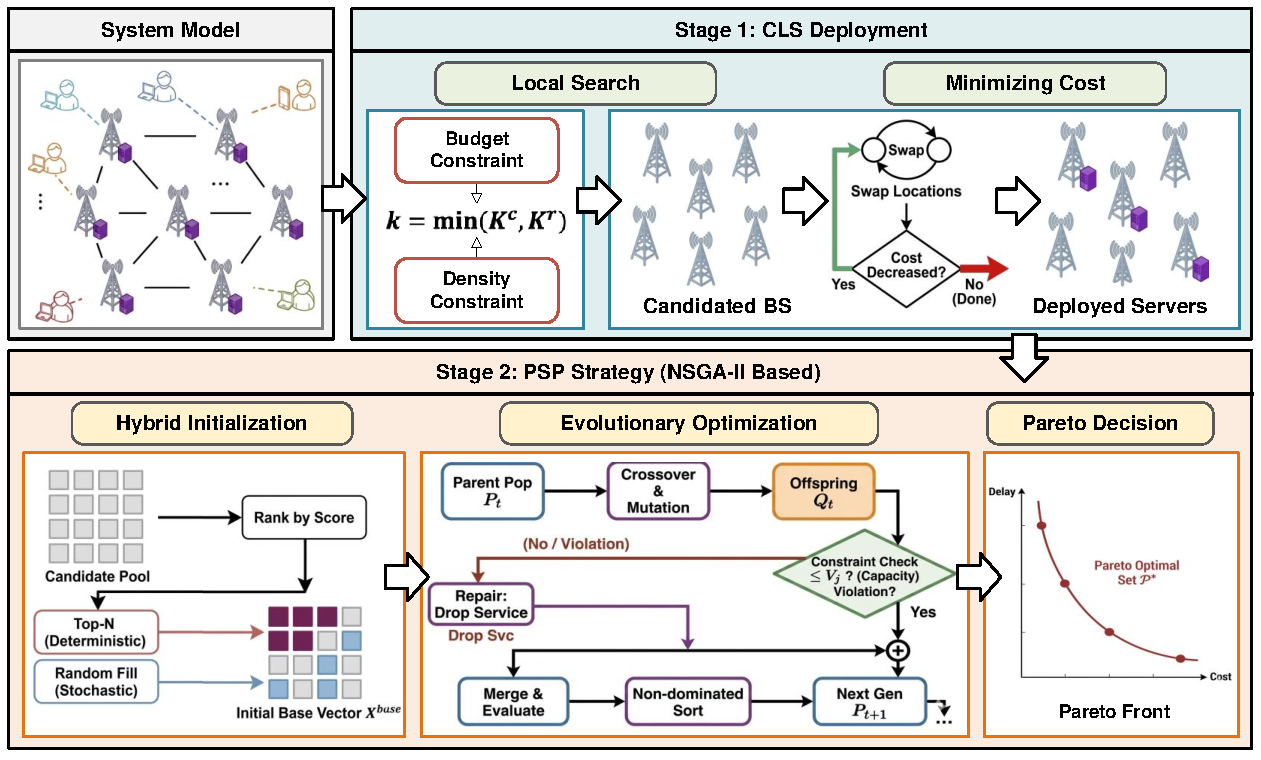
\includegraphics[width=1.8\columnwidth]{algo_0421.pdf}
    \caption{Overall architecture of MOS\textsuperscript{2}.}
    \label{fig:algo}
\end{figure*}

\section{Algorithm Design}
In this section, we present a staged decision-making process that captures server deployment decisions based on user density distribution and operator budget, and supports a latency and cost-aware service provisioning mechanism. Our strategy aims to minimize deployment and transmission costs during these two stages from the perspective of mobile network operators, and to jointly optimize the provisioning cost and user-perceived latency in the subsequent service provisioning stage.

% ==================== 新增的总体框架解释 (微调版) ====================
To systematically illustrate our proposed approach, Fig.~\ref{fig:algo} depicts the overall architecture of the multi-stage joint optimization framework. The problem is logically decoupled into two primary interconnected stages:

\textbf{1) Stage 1: CLS-based Server Deployment.} 
 Building on the system model established above, Stage 1 is triggered to determine the optimal placement of edge servers.
  Initially, the exact number of deployable servers is rigorously derived by jointly evaluating the operator's budget
  constraints and the user density requirements. Subsequently, a Coverage-based Local Search (CLS) algorithm is executed
  among the candidate base stations. Through an iterative "Swap" mechanism, the algorithm continuously evaluates and
  minimizes the total deployment and transmission cost. The loop terminates when no further cost decrease can be achieved,
  outputting a fixed set of deployed server locations. This spatial configuration acts as a fundamental physical constraint
  for the subsequent phase.


\textbf{2) Stage 2: PSP Strategy for Service Provisioning.}
Given the fixed server locations, PSP constructs a hybrid initial population and applies NSGA-II to optimize provisioning cost and access delay. Crossover and mutation produce each offspring, whose entries are first rounded to binary values. For every server $m_j$, PSP then checks $\sum_w z_{jw}\leq V_j$. If the capacity is exceeded, selected service entries are randomly deactivated until feasibility is restored. Only capacity-feasible offspring are evaluated and passed to non-dominated sorting; thus, feasibility is enforced by repair rather than by a penalty function. The evolutionary process returns a set of provisioning schemes representing different cost--delay trade-offs.

% =========================================================



%%%%%%%%Xu:下面这行是本节的开头段，需要翻译。
%我们提出的策略可以在服务器放置阶段对放置成本和传输成本做出优化，并在后续的服务部署阶段对服务部署的成本与用户延迟进行联合优化。
\addtolength{\topmargin}{0.06in}
\begin{algorithm}[!t]
    \caption{Coverage-based Local Search (CLS)}
    \label{algo:local_search}
    \KwIn{$\mathcal{M}$, $\mathcal{U}$, $k$, $r$, $T_{\max}$}
    \KwOut{$\mathcal{S}$, $C$}
    $\mathcal{S} \leftarrow \textbf{RandomSelect}(\mathcal{M},k)$\;
    $C \leftarrow \textbf{ComputeCost}(\mathcal{S}, \mathcal{U}, r)$\;
    $t \leftarrow 0$\;

    \While{$t < T_{\max}$}{
        $\Delta \leftarrow \textbf{False}$\;

        \ForEach{$i \in \mathcal{S}$}{
            \ForEach{$j \in \mathcal{M} \setminus \mathcal{S}$}{
                $\mathcal{S}' \leftarrow \mathcal{S} \setminus \{i\} \cup \{j\}$\;
                $C' \leftarrow \textbf{ComputeCost}(\mathcal{S}', \mathcal{U}, r)$\;

                \If{$C' < C $}{
                    $\mathcal{S} \leftarrow \mathcal{S}'$\;
                    $C \leftarrow C'$\;
                    $\Delta \leftarrow \textbf{True}$\;
                    \textbf{break}\;
                }
            }
            \If{$\Delta$}{\textbf{break}}
        }

        \If{\textbf{not} $\Delta$}{\textbf{break}}

        $t \leftarrow t + 1$\;
    }

    \KwRet{$\mathcal{S}, C$}
\end{algorithm}

\subsection{Server Deployment Optimization: CLS}
%%%%%%这里应该是budget-based solution的一个部分
In the first stage, we focus on optimizing the deployment of edge servers to support diverse services in dynamic edge environments and to assist mobile network operators in making informed placement decisions. Considering the distribution of user demand and budget constraints, this stage seeks to identify efficient server locations that maximize service coverage and system performance. 


We reformulate server deployment as a facility-location problem in which candidate base stations are potential server sites and users are demand points with heterogeneous service requirements. The deployment budget $C_{\max}$ gives the upper bound $\mathcal{K}^c=\left\lfloor C_{\max}/\min_j\{p_j\}\right\rfloor$ on the number of deployable servers. For each candidate base station $b_k$, we compute the user density $\sigma_k$ within a circular coverage region of radius $r$. Let $\mathcal{K}^r=\sum_{b_k\in\mathcal{B}}\mathbf{1}_{\{\sigma_k\geq\sigma_{\min}\}}$ denote the number of candidate sites whose local density reaches threshold $\sigma_{\min}$. The target server count is then $k=\min\{\mathcal{K}^c,\mathcal{K}^r\}$, reflecting both budget feasibility and the spatial distribution of demand.

Based on this estimate, we achieve an initial optimization of the deployment cost $C_d(m_j)$. We then optimize the transmission cost $C_t(m_j)$ and integrate it into a classical location problem by using the $k$-median formulation. Specifically, given a set of candidate server locations where each server can serve a certain number of users, the objective is to select $k$ base stations that deploy the servers in such a way that the total distance between each user and the nearest server is minimized. The detailed steps are outlined in Algorithm~\ref{algo:local_search}.
%本段末尾再补一句，为下面第一行。
%%%%%%Xu:
%我们通过对$\widetilde{\mathcal{K}}的抉择实现了对放置成本$C_{d}(m_j)$的优化。
%在确定了放置成本$C_{d}(m_j)$之后，我们下一步将对传输成本$C_{t}(m_j)进行优化。本文将原始的边缘网络服务节点放置问题转化为工厂选址问题，选择K-median作为设施放置场景。具体而言，本研究当前有一个候选服务器集合，每个服务器可以服务一定数量的用户，其优化目标是选择K个服务器部署位置，使得这些服务器能够最小化所有用户到其最近的服务器的总距离。因此，上一部分中确定的预计部署服务器的数量$\widetilde{\mathcal{K}}即为该问题下的k值。在k值确定后，本节将使用局部搜索策略解决问题。该策略会首先随机选择k个基站作为待部署服务器的基站，然后通过不断交换当前选择的基站和候选集合中的其他未选中的基站来减少用户与候选服务器间的物理距离。由于在Transmission Cost中我们提到物理距离与传输成本密切相关，因此我们通过最小化所有用户到其最近的服务器的总距离来实现对$C_{t}(m_j)的优化。
%下面是伪代码以及解释
% Pseudocode for Generate Initial Population
\begin{algorithm}[!t]
    \caption{Initial Base Configuration (\texttt{IBC} ($\alpha$, $\beta$, $\varpi_j$))}
    \label{alg:init_pop_hybrid}
    \KwIn{$\mathcal{M}$, $\mathcal{U}$, $\mathcal{S}$, $k$, $V_j$,  $\alpha$, $\beta$, $\varpi_j$}
    \KwOut{$X^{base}$}
    Initialize $X^{base} \leftarrow \mathbf{0}$\;
    \For{$j \leftarrow 1$ \KwTo $k$}{
        $C_j^{cost} \leftarrow \textbf{CostGreedyCandidates}(j)$;\\
        $C_j^{delay} \leftarrow \textbf{DelayGreedyCandidates}(j)$;\\ 
        Construct set $C_j \leftarrow C_j^{cost} \cup C_j^{delay}$;

        \ForEach{$s_w \in C_j$}{
            % $H(s_w) \leftarrow \alpha\,w_{cost}(s) + \beta\,w_{delay}(s)$
            Calculate the hybrid score $H_j(s_w)$;
        }
        Sort $C_j$ by descending $H_j(s_w)$;\\
        % Check capacity and select services
        \If{$|C_j| > V_j$}{
            % $A_j \leftarrow$ top $\lfloor\alpha \cdot m\rfloor$ services from $C_j$,
            % $A_j \leftarrow \textbf{Top-N}(C_j,\lfloor\alpha \cdot \varpi_j\rfloor)$;\\
            % $R_j \leftarrow$ randomly select $(V_j - \lfloor\alpha \cdot \varpi_j\rfloor)$ services from $C_j \setminus A_j$
            % $R_j \leftarrow \textbf{Select}(C_j,V_j - \lfloor\alpha \cdot \varpi_j\rfloor)$;\\  
            $A_j \leftarrow \textbf{Top-N}(C_j, \varpi_j)$;\\
            $R_j \leftarrow \textbf{Select}(C_j \setminus A_j,\; V_j - \varpi_j)$;\\
            $L_j \leftarrow A_j \cup R_j$;\\
        }
        \Else{
            $L_j \leftarrow C_j$;
        }

        Set row $j$ of $X^{base}$ to the indicator vector of $L_j$
    }

    \Return $X^{base}$
\end{algorithm}

% To begin, several preparatory elements are required for the algorithm, including the set of candidate server positions denoted by $\mathcal{M}$, representing all potential deployment locations for the servers; the set of user positions $\mathcal{U}$; the number of servers $k$, representing the number of servers to be selected; the coverage radius $r$, used to calculate the service coverage area of each server; and the maximum number of iterations $T_{\max}$, which controls the termination condition of the algorithm. 
% In line 1, the algorithm randomly selects $k$ positions from the candidate position set $\mathcal{M}$ to form the initial server deployment $\mathcal{S}$. It then computes the communication cost $C$ for the initial solution, based on the current server deployment $\mathcal{S}$, user positions $\mathcal{U}$, and the coverage radius $r$ in line 2. In lines 4-20, the algorithm enters the iterative optimization phase. Starting from line 5, for each server position $i \in \mathcal{S}$, it attempts to replace $i$ with a candidate position $j \in \mathcal{M} \setminus \mathcal{S}$ that has not been selected, generating a new solution \(\mathcal{S}' = \mathcal{S} \setminus \{i\} \cup \{j\}\). 
% The communication cost \(C'\) for the new solution is calculated in line 9. In lines 10–12, if $C'$ is lower than the current cost $C$, indicating an improvement, the new solution is accepted, and the current deployment and cost are updated as $\mathcal{S} \leftarrow \mathcal{S}'$ and $C \leftarrow C'$. Subsequently, the algorithm checks whether any improvement was found in the current iteration in lines 14-16. If no improvement is found or the maximum number of iterations $T_{\max}$ is reached, the algorithm terminates. Finally, in line 21, the algorithm returns the server deployment $\mathcal{S}$ with the minimum communication cost and the corresponding minimal cost $C$.
%整合优化语言
To begin, several preparatory elements are required for the algorithm: the candidate server position set
  $\mathcal{M}$, representing all potential deployment locations; the user position set $\mathcal{U}$; the target number
   of servers $k$ to be selected; the coverage radius $r$, used to calculate the service coverage area of each server;
  and the maximum number of iterations $T_{\max}$, which controls the termination condition of the algorithm.

  In line 1, the algorithm randomly selects $k$ positions from $\mathcal{M}$ to form the initial server deployment
  $\mathcal{S}$, and line 2 computes the corresponding communication cost $C$ over $\mathcal{U}$ under the coverage
  radius $r$. Lines 4--19 then enter the iterative optimization phase. For each server position $i \in \mathcal{S}$, the
   algorithm attempts to replace $i$ with a non-selected candidate $j \in \mathcal{M} \setminus \mathcal{S}$, generating
   a new solution $\mathcal{S}' = \mathcal{S} \setminus \{i\} \cup \{j\}$, and its communication cost $C'$ is calculated
   in line 9. In lines 10--14, if $C' < C$, indicating an improvement, the new solution is accepted and the current
  deployment and cost are updated as $\mathcal{S} \leftarrow \mathcal{S}'$ and $C \leftarrow C'$. Lines 17--18 then
  check whether any improvement was found in the current iteration; if no cost-reducing swap exists or $T_{\max}$ is
  reached, the algorithm terminates. Finally, in line 20, the algorithm returns the server deployment $\mathcal{S}$ with
   the minimum communication cost and the corresponding minimal cost $C$.

%加一段算法时间复杂度分析
The computational complexity of Algorithm~1 is $O(T_{\max} \cdot k \cdot |\mathcal{M}| \cdot |\mathcal{U}|)$. Within
  each iteration, for every server slot $i \in \mathcal{S}$ the algorithm examines at most $|\mathcal{M}| - k$ candidate
   replacements $j \in \mathcal{M} \setminus \mathcal{S}$, and every invocation of $\textbf{ComputeCost}(\cdot)$
  aggregates the coverage distances over all $|\mathcal{U}|$ users in $O(|\mathcal{U}|)$ time. The per-iteration cost is
   therefore $O(k \cdot |\mathcal{M}| \cdot |\mathcal{U}|)$, and the outer loop runs at most $T_{\max}$ times, yielding
  the stated bound. In practice the early-termination flag $\Delta$ exits the loop as soon as no cost-reducing swap can
  be found, so the observed runtime is substantially lower than this worst-case expression. Since $T_{\max}$ is a small
  constant and $k \ll |\mathcal{M}|$ in realistic MEC deployments, Algorithm~1 scales linearly in the product of the
  candidate-pool size and the user population, which guarantees tractability at city-scale.



% Main PSP Algorithm with Initial Population Call
\begin{algorithm}[!t]
    \caption{Pareto-based Service Provisioning (PSP)}
    \label{algo:nsga2_deploy}
    \KwIn{$\mathcal{M}$, $\mathcal{U}$, $\mathcal{S}$, $k$, $G$, $N$, $V_j$, $\alpha$, $\beta$, $\varpi_j$}
    \KwOut{$\mathcal{P}^*$}

    % Initialize base matrix via the hybrid greedy function
    % $X^{base} \leftarrow IBC(k, \mathcal{S}, c, \alpha, \beta, m)$
    $X^{base} \leftarrow$ $\texttt{IBC}$ ($\alpha$, $\beta$, $\varpi_j$);\\
    % Generate and evaluate initial population
    Generate initial population $\mathcal{P}$ of size $N$ by stochastic bit-flip perturbation around $X^{base}$ \;
    \ForEach{$X \in \mathcal{P}$}{
        Round and reshape $X$ to $k \times |\mathcal{S}|$\;
        For each row $j$, randomly deactivate selected entries while $\sum_w X_{jw}>V_j$\;
        Evaluate objectives $C_{p}(m_j)$ and $\mathbb{D}(m_j)$\;
    }
    % Evolutionary loop
    \For{$g \leftarrow 1$ \KwTo $\mathrm{G}$}{
        Non-dominated sort $\mathcal{P}$ and assign crowding distances\;
        Select parents via tournament selection\;
        Apply crossover and mutation to produce offspring $\mathcal{P}'$\;
        \ForEach{$X' \in \mathcal{P}'$}{
            Round and reshape $X'$; repair each violating row as above; evaluate $X'$;% as above\;
        }
        $\mathcal{P} \leftarrow \textbf{Top-N}(\mathcal{P} \cup \mathcal{P}', N)$\;
    }

    \KwRet{$\mathcal{P}^*$}
\end{algorithm}
%首先，算法需要若干输入元素，包括候选服务器位置集合 \(\mathcal{C}\)，表示所有可能部署服务器的候选点；用户位置集合 \(\mathcal{U}\)，反映用户分布情况；服务器部署数量 \(k\)，即需要选取的服务器数量；覆盖半径 \(r\)，用于计算服务器的服务覆盖范围；以及最大迭代次数 \(T_{\max}\)，用于控制算法终止条件。
%在第1行，算法随机从候选位置集合 \(\mathcal{C}\) 中选择 \(k\) 个位置，构造初始服务器部署方案 \(\mathcal{S}\)。第2行计算该初始方案下的通信成本 \(C\)，该成本基于当前服务器部署方案 \(\mathcal{S}\)、用户位置 \(\mathcal{U}\) 及覆盖半径 \(r\) 计算得出。第3行初始化迭代计数器 \(t\) 为0。
%在第4至20行，算法进入迭代优化阶段。第5行开始，针对当前方案 \(\mathcal{S}\) 中的每一个服务器位置 \(i\)，第6行尝试用候选位置集合中尚未选取的位置 \(j \in \mathcal{C} \setminus \mathcal{S}\) 进行替换，形成新方案 \(\mathcal{S}' = \mathcal{S} \setminus \{i\} \cup \{j\}\)。第8行对新方案计算通信成本 \(C'\)。第9至12行如果新方案通信成本 \(C'\) 低于当前成本 \(C\)，表明方案有所改进，则接受新方案并更新当前方案与成本，即 \(\mathcal{S} \leftarrow \mathcal{S}'\)，\(C \leftarrow C'\)。
%如果在当前迭代中未发现任何改进或达到最大迭代次数，算法终止。最终，在第21行，算法返回通信成本最低的服务器部署方案 \(\mathcal{S}\) 及对应的最小通信成本 \(C\)。
\begin{figure*}[!t]
	\centering
	\addtolength{\subfigcapskip}{-2pt}
 %    \subfigure[\# edge servers and users (10, 180).]
	% {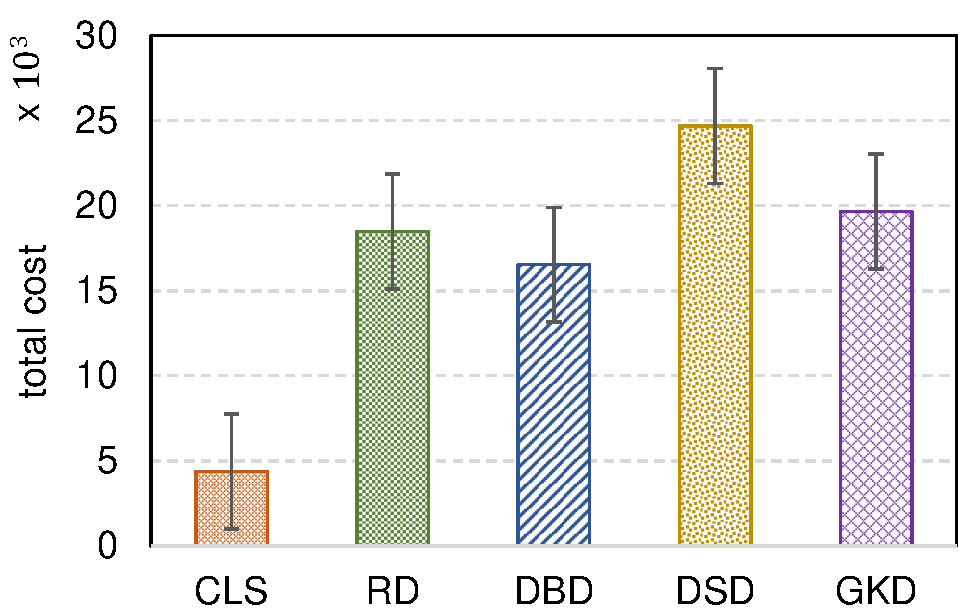
\includegraphics[width=1.75in]{s10-u180_new.pdf}}
	% \subfigure[\# edge servers and users (20, 180).]
	% {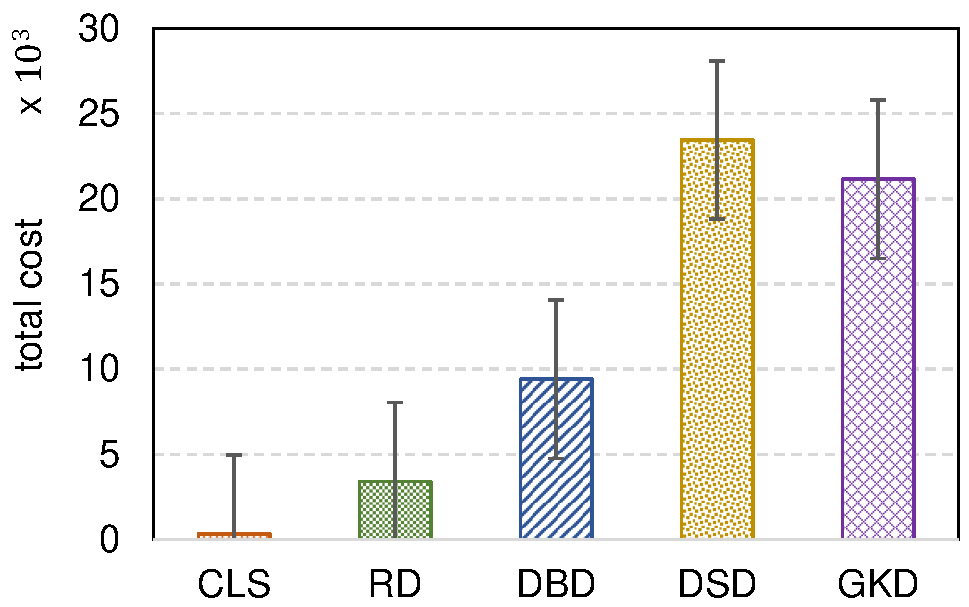
\includegraphics[width=1.75in]{s20-u180_new.pdf}}
	% \subfigure[\# edge servers and users (10, 300).]
	% {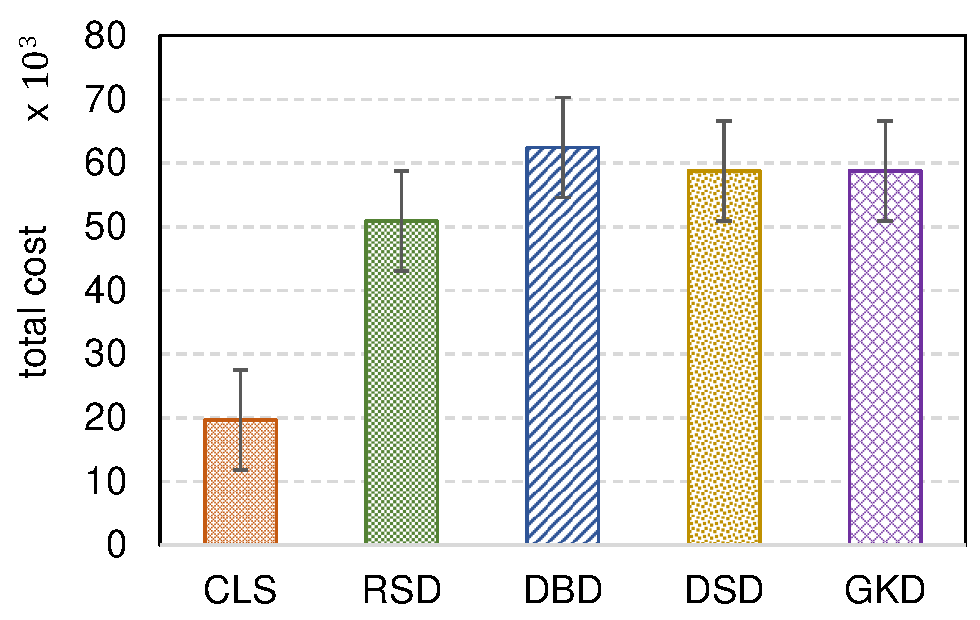
\includegraphics[width=1.75in]{s10-u300_new.pdf}}
	% \subfigure[\# edge servers and users (20, 300).]
	% {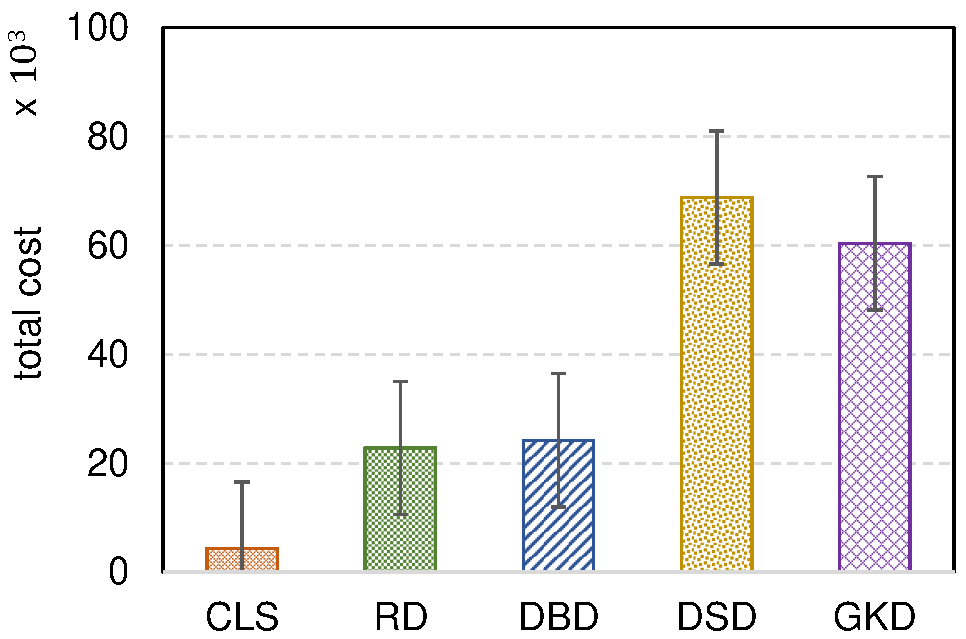
\includegraphics[width=1.70in]{s20-u300_new.pdf}}
 %    \vspace{-5pt}
	% \caption{Performance of server deployment (stage one) by considering different numbers of edge servers and users.} 
	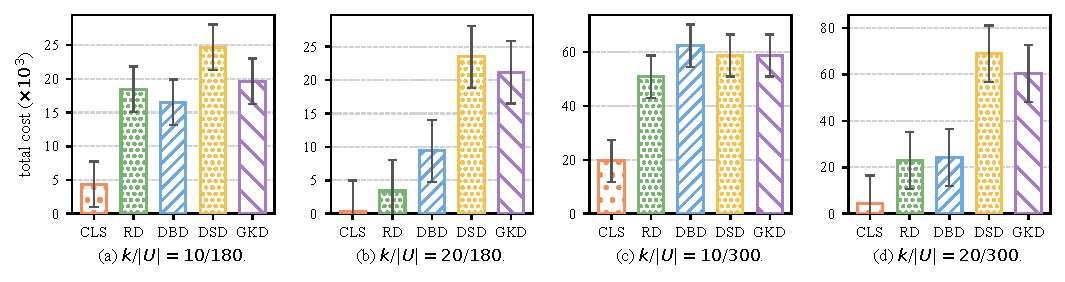
\includegraphics[width=\textwidth]{stage1_scale_comparison_readable.pdf}
	\caption{Stage-I server-deployment performance under different server and user scales.}
	\label{fig2}
    \vspace{-7pt}
\end{figure*}

\begin{figure}[!t]
	\centering
	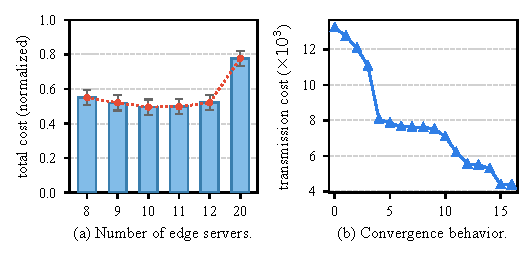
\includegraphics[width=\columnwidth]{stage1_cost_analysis_readable.pdf}
	\caption{Stage-I cost analysis under varying server counts and CLS iterations.}
	\label{fig_compare}
    \vspace{-7pt}
\end{figure}
\begin{figure*}[!t]
	\centering
	
\includegraphics[width=\textwidth]{stage2_fixed_servers_with_dqn_clean.pdf}
	\caption{Service-provisioning performance with 10 deployed servers and increasing user populations.}
	\label{fig4}
\end{figure*}

\subsection{Pareto-based Service Provisioning - PSP}
After determining the number and locations of deployed servers in the first stage, we proceed to address service provisioning on these servers to meet actual user demands. According to $\textbf{P}_3$, the functions $\mathbb{D}(m_j)$ and $C_{p}(m_j)$ remain undetermined at this stage. Therefore, we propose a Pareto-based strategy to jointly optimize cost and delay by deploying diverse services to selected servers while satisfying capacity constraints, thereby solving the service provisioning problem under fixed server locations.


A service-provisioning scheme is encoded by a binary matrix $\textit{indiv}\in\{0,1\}^{k\times|\mathcal{S}|}$. Each row corresponds to a deployed server and each column to a service type. The entry $\textit{indiv}[j,w]$ is the encoded counterpart of $z_{jw}$: it equals $1$ when service $s_w$ is provisioned on server $m_j$, and $0$ otherwise. The provisioning cost on $m_j$ is
\begin{equation}
C_{p}(m_j)=\sum_{w\in\mathcal{S}}\textit{indiv}[j,w]sc_w.
\end{equation}
To ensure that no server exceeds its capacity, the encoding satisfies
\begin{equation}
\sum_{w \in \mathcal{S}} \textit{indiv}[j, w] \leq V_j, \quad \forall j \in \mathcal{M}.
\end{equation}


After crossover and mutation, every encoded entry is rounded to $0$ or $1$. If $\sum_w \textit{indiv}[j,w]>V_j$ for any server $j$, selected entries in that row are randomly set to $0$ until the capacity constraint is satisfied. Objective evaluation and non-dominated sorting are then performed on the repaired feasible individual.



PSP uses a hybrid initialization before the NSGA-II evolutionary loop. For each server, it constructs one ranking that favors low provisioning cost and another that favors services requested frequently by locally assigned users. The two rankings are fused by a hybrid score. High-scoring services form a deterministic anchor set, and the remaining capacity is filled by stochastic sampling from lower-ranked candidates. The resulting base configuration combines exploitation of high-quality candidates with exploration of alternative service combinations.

% Definition for Generate Initial Population (Hybrid Greedy)

\begin{definition}[hybrid score]\label{def:init_pop}
Let $\alpha,\beta\in[0,1]$ balance provisioning cost and local demand, with $\alpha+\beta=1$. Let $\varpi_j$ $(0<\varpi_j\leq V_j)$ denote the deterministic anchor size on edge server $m_j$. The hybrid score of candidate service $s_w$ is
\begin{equation}
H_j(s_w)=\alpha w_{\mathrm{cost},j}(s_w)+\beta w_{\mathrm{req},j}(s_w),
\label{eq:hybrid_score}
\end{equation}
where $w_{\mathrm{cost},j}$ and $w_{\mathrm{req},j}$ are descending rank scores derived from provisioning cost and the request frequency of users assigned to $m_j$, respectively. We set $\varpi_j=\lceil\rho V_j\rceil$ with $\rho=0.5$, reserving half of the capacity for high-ranked deterministic services and half for stochastic selection from the remaining candidates.
\end{definition}


% For each server \(j\), candidate services are ranked in descending order of their hybrid scores. If the ranked list contains no more than the per-server capacity $V_j$, all candidates are deployed. Otherwise, the top $\alpha \cdot \varpi_j$ services form the Top-N anchor set $A_j$, and the remaining $V_j-\alpha \cdot \varpi_j$ slots are filled by randomly sampling from the random-fill set $R_j$. The final selection for each server $j$ constitutes the $j$-th row of the base matrix $X^{\mathrm{base}}$, which serves as the hybrid seed for initializing the population in the evolutionary optimization process. 
%优化表述，描述算法2过程
Line~1 of Algorithm~\ref{alg:init_pop_hybrid} initializes the base matrix $X^{\mathrm{base}}$ to a zero
  matrix, and the outer loop in lines 2--15 builds one row per deployed server. For each server $j$, lines 3--5
  construct the candidate pool $C_j$ by taking the union of two greedy rankings: the cost-oriented ranking
  $C_j^{\mathrm{cost}}$ returned by $\textbf{CostGreedyCandidates}(j)$ and the delay-oriented ranking
  $C_j^{\mathrm{delay}}$ returned by $\textbf{DelayGreedyCandidates}(j)$. Lines 6--7 then evaluate the hybrid
  score $H_j(s_w)$ defined in Eq.~\eqref{eq:hybrid_score} for every candidate service $s_w \in C_j$, and line~8
  sorts $C_j$ in descending order of $H(\cdot)$. Lines 9--14 perform the capacity-aware selection: if $|C_j|$
  exceeds the per-server capacity $V_j$, the top $\varpi_j$ services form the deterministic anchor set $A_j$
  (line~10, $\textbf{Top-N}$), while the remaining $V_j - \varpi_j$ slots are filled by randomly sampling from
  the lower-ranked remainder $C_j \setminus A_j$ (line~11, $\textbf{Select}$); otherwise all candidates are
  retained as $L_j = C_j$ (line~14). Line~15 converts $L_j$ into an indicator vector and writes it to the $j$-th
   row of $X^{\mathrm{base}}$, and line~16 returns the assembled base matrix, which serves as the hybrid seed
  for the subsequent evolutionary optimization.


Figure~\ref{fig:hybrid_init} illustrates the construction for Server~0. Panel~(a) decomposes each candidate's hybrid score into cost- and request-oriented components, and panel~(b) shows the deterministic anchor, stochastic fill, and discarded candidates under the capacity limit.


During optimization, each individual represents a service deployment scheme encoded as a binary vector $X = [x_1, x_2, \dots, x_{k \cdot |\mathcal{S}|}]$ where $x_i \in \{0,1\}$ indicates the deployment state at position $i$. Individuals are evaluated against two objectives: deployment cost $C_p(m_j)$ and access delay $\mathbb{D}(m_j)$. The algorithm first performs non-dominated sorting, prioritizing individuals by dominance rank. For equal-rank individuals, crowding distance comparison serves as the secondary selection criterion. Population updating employs classical crossover and mutation operators to expand the solution space. Crossover combines two parent individuals by exchanging gene segments at random points, while mutation randomly flips deployment states ($0 \leftrightarrow 1$) in vector $X$, abstracted as $X'= \texttt{mutation} (X)$. 


Each generation merges the parent and offspring populations and retains $N$ individuals according to non-dominated rank and crowding distance. At generation $G$, PSP returns the non-dominated capacity-feasible provisioning schemes found by the search. The detailed steps are outlined in Algorithms~\ref{alg:init_pop_hybrid} and~\ref{algo:nsga2_deploy}.


The normalized score $Q$ is applied after optimization to select one balanced solution for scalar comparison; it is not an objective used to generate the Pareto population.

%%%%第二部分开始
%在Stage I确定好了部署服务器的数量和位置之后，我们需要继续考虑如何在服务器上部署服务以满足实际用户服务需求。根据&\textbf{P}_3,此阶段的还没有确定的函数为\mathbb{D}(m_j),和C_{p}(m_j)。因此，本文采用NSGA-II算法，在满足服务器容量限制的情况下，将不同类型的服务部署到选定的服务器上来对成本与延迟进行联合优化，解决固定服务器选址情况下的服务部署问题。
%在本研究中，服务部署方案采用一个二进制矩阵 $\textit{indiv}$ 进行表示。设系统包含 $k$ 台服务器和 $|\mathcal{S}|$ 类服务，则该部署矩阵大小为 $k \times |\mathcal{S}|$，其中每一行对应一台服务器，每一列对应一种服务类型。矩阵中第 $j$ 行第 $w$ 列的元素 $\textit{indiv}[j, w]$ 为 $0$ 或 $1$，表示是否在第 $j$ 台服务器上部署了第 $w$ 类服务，即当 $\textit{indiv}[j, w] = 1$ 时，表示该服务被部署；若为 $0$，则表示未部署。在此部署方案基础上，服务部署总成本可细化表示为：

% \begin{equation}
% C_{p}(m_j) = \sum_{w \in \mathcal{S}} \sum_{j \in \mathcal{M}} \textit{indiv}[j, w] \cdot sc[w]
% \end{equation}

%为了保证每台服务器的部署容量不超过系统预设的最大值，设每台服务器允许部署的最大服务数量为 $V_j$，通过以下约束条件加以限制：

% \begin{equation}
% \sum_{w \in \mathcal{S}} \textit{indiv}[j, w] \leq V_j, \quad \forall j \in \mathcal{M}
% \end{equation}

%若在部署过程中某台服务器上服务数量超过容量限制，则采用修复策略，随机移除部分已部署服务（即将对应的 $\textit{indiv}[j, w]$ 设置为 $0$），直到满足约束。
%本文在生成初始种群时对基础NSGA-II算法做出了改进，将随机初始化种群，改为基于服务成本和请求延迟的贪心策略混合方案。该方案会根据成本和延迟混合出一组服务部署方案，然后从该方案中先选择一部分优化程度较好的服务，再从剩下的服务中随机选择另一部分将其合并作为新的初始解。利用该初始解生成算法的初始种群，并进行后续的优化。在优化过程中，种群中的每个个体对应一个服务部署方案，其编码形式为一维二进制向量 $X = [x_1, x_2, \dots, x_{k \cdot |\mathcal{S}|}]$，其中 $x_i \in {0,1}$ 表示第 $i$ 个服务部署位的状态。每个个体被同时评估两个目标函数：部署成本 $C_p(m_j)$ 与访问延迟 $\mathbb{D}(m_j)$。算法首先对种群进行非支配排序，并将所有个体按其支配等级划分，等级较低者优先被选择。对于同一等级的个体，使用拥挤度比较进行次级选择。在种群更新过程中，系统采用经典的交叉与变异操作扩展解空间。交叉操作通过选取两个父代个体，在随机交叉点交换其部分基因生成新个体；变异操作则随机翻转某些位置的部署状态，即对解向量 $X$ 中任意位置进行 $0 \leftrightarrow 1$ 的切换，其形式可抽象表示为：
% \begin{equation}
% X_{\text{new}} = \text{mutation}(X)
% \end{equation}
%最终，在每一代中，算法通过将父代和子代合并并重新排序，选出前 $N$ 个最优个体进入下一代，从而确保收敛性与解集多样性。迭代过程持续至最大代数限制，最终输出一组满足部署容量约束的 Pareto 最优服务部署方案，以及在加权目标函数下的最优联合开销结果。
%参考wushen论文的definition 为伪代码里的参数作出定义；2-9单拎出来，用function，algorithm1:Generate initial population(定义一个方法名)，然后这个代码里直接写成调用的形式
% Let \(\mathcal{M}\) be the set of candidate server positions,
% \(\mathcal{U}\) the set of user positions,
% \(\mathcal{S}\) the catalog of service types,
% \(k=|\mathcal{M}|\) the number of servers to be deployed.
% % Updated descriptive paragraph
% Then, in Algorithm \ref{algo:nsga2_deploy}, lines 1–2 invoke Algorithm 2 to generate an initial population routine to construct the base configuration using our hybrid greedy strategy. Lines 3–6 generate an initial population by perturbing this base, followed by rounding, capacity repair, and objective evaluation for each individual. The main evolutionary loop (lines 7–14) performs non-dominated sorting, crowding distance assignment, selection, crossover, mutation, and repair/evaluation of offspring, and merges populations to retain the top $N$ solutions. Finally, the Pareto-optimal set $\mathcal{P}^*$ is returned, representing the best trade-offs between cost and delay across all generations.
% %加一段时间复杂度分析
% The overall complexity of the proposed PSP (Algorithm~3) is $O\!\left(G \cdot \bigl(N^{2} + N \cdot (k \cdot |\mathcal{S}|
%    + |\mathcal{U}|)\bigr)\right)$, where $G$ is the maximum number of generations, $N$ the population size. The Initial
%   Base Configuration (Algorithm~2) is executed exactly once before the evolutionary loop: for each of the $k$ servers we
%   build the cost-oriented and delay-oriented greedy rankings and evaluate the hybrid score $H(s_{w})$ in $O(|\mathcal{S}|)$,
%    sort the candidate set $C_{j}$ by $H(\cdot)$ in $O(|\mathcal{S}| \cdot \log |\mathcal{S}|)$, and perform the Top-$N$
%   anchor selection together with the random fill in $O(|\mathcal{S}|)$; therefore IBC contributes a one-time cost of $O(k
%   \cdot |\mathcal{S}| \cdot \log |\mathcal{S}|)$. Inside the evolutionary loop, each generation performs non-dominated
%   sorting and crowding-distance assignment in $O(N^{2})$, constraint-aware repair and bi-objective evaluation in $O(k \cdot
%   |\mathcal{S}| + |\mathcal{U}|)$ per individual, and elitist truncation in $O(N \cdot \log N)$.

%整合优化新版

Let $\mathcal{M}$ be the set of deployed servers obtained from Stage~1, let $\mathcal{U}$ be the set of user positions, let $\mathcal{S}$ be the service catalog, and let $k=|\mathcal{M}|$ be the number of deployed servers.

  % Updated descriptive paragraph
  Then, in Algorithm~\ref{algo:nsga2_deploy}, line~1 invokes Algorithm~2 (IBC) to construct a base configuration
  $X^{\text{base}}$ using our hybrid greedy strategy, and line~2 generates the initial population $\mathcal{P}$ of size
  $N$ by binary perturbation around $X^{\text{base}}$. Lines 3--6 then round every individual, apply capacity repair,
  and evaluate its bi-objective values $C_{p}(m_{j})$ and $\mathbb{D}(m_{j})$. The main evolutionary loop (lines 7--14)
  performs non-dominated sorting with crowding-distance assignment, selects parents via tournament, applies crossover
  and mutation to produce offspring, repairs and evaluates them, and merges parent and offspring populations to retain
  the top $N$ individuals for the next generation. Finally, the Pareto-optimal set $\mathcal{P}^{*}$ is returned,
  representing the best cost--delay trade-offs found across all generations.

  %加一段时间复杂度分析
  The overall complexity of the proposed PSP (Algorithm~3) is $O\!\left(G \cdot \bigl(N^{2} + N \cdot (k \cdot
  |\mathcal{S}| + |\mathcal{U}|)\bigr)\right)$, where $G$ is the maximum number of generations and $N$ the population
  size. The Initial Base Configuration (Algorithm~2) is executed exactly once before the evolutionary loop: for each of
  the $k$ servers we build the cost-oriented and delay-oriented greedy rankings and evaluate the hybrid score $H(s_{w})$
   in $O(|\mathcal{S}|)$, sort the candidate set $C_{j}$ by $H(\cdot)$ in $O(|\mathcal{S}| \cdot \log |\mathcal{S}|)$,
  and perform the Top-$N$ anchor selection together with the random fill in $O(|\mathcal{S}|)$; therefore IBC
  contributes a one-time cost of $O(k \cdot |\mathcal{S}| \cdot \log |\mathcal{S}|)$. Inside the evolutionary loop, each
   generation performs non-dominated sorting and crowding-distance assignment in $O(N^{2})$, constraint-aware repair and
   bi-objective evaluation in $O(k \cdot |\mathcal{S}| + |\mathcal{U}|)$ per individual, and elitist truncation in $O(N
  \cdot \log N)$. Because the IBC cost is strictly dominated by the evolutionary term under realistic population sizes, the hybrid initialization preserves the asymptotic complexity of a standard NSGA-II while empirically tightening the effective search space.

\begin{figure}[!t]
	\centering
	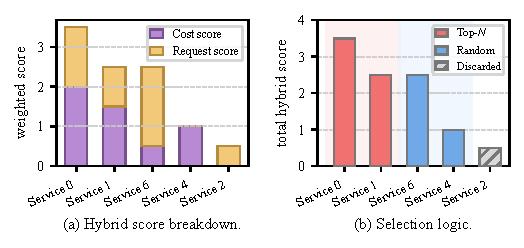
\includegraphics[width=\columnwidth]{hybrid_initialization_readable.pdf}
	\caption{Hybrid initialization for candidate services on Server~0.}
	\label{fig:hybrid_init}
    \vspace{-7pt}
\end{figure}

% \begin{algorithm}[!t]
%     \caption{Pareto-based Service Provisioning (PSP)}
%     \label{algo:nsga2_deploy}
%     \KwIn{$\mathcal{M}$ (server positions), $\mathcal{U}$ (user positions), $\mathcal{S}$ (service types), $k$ (number of servers), $c$ (service capacity limit for provision),$\mathcal{A}$ (user-to-server assignments)}
%     \KwOut{$\mathcal{P}^*$ (Pareto-optimal service deployment plans)}

%     Initialize base deployment matrix $X^{base}$ as a $k \times |\mathcal{S}|$ binary matrix\;

%     \For{$j \leftarrow 1$ \KwTo $k$}{
%         Obtain candidate service sets $C_j^{cost}$ and $C_j^{req}$ using cost-based and request-based greedy strategies\;
%         Compute score for each service $s \in C_j^{cost} \cup C_j^{req}$ as:\;
%         \Indp
%         $score(s) = \alpha \cdot w_{cost}(s) + \beta \cdot w_{req}(s)$, where $w_{cost}$ and $w_{req}$ are weights based on service ranking\;
%         \Indm
%         Sort all services by descending score\;
%         %$\alpha \cdot m$ 向下取整
%         Select top $\alpha \cdot m$ services as anchor set $A_j$\;
%         Randomly select $(c - \alpha \cdot m)$ services from the remaining candidates to form $R_j$\;
%         Set row $j$ of $X^{base}$ as $A_j \cup R_j$\;
%     }

%     Generate initial population $\mathcal{P}$ of $N$ individuals by applying binary perturbation on $X^{base}$\;
%     %for each这里再考虑一下 表示每个Popsize下的种群
%     \ForEach{ $X \in \mathcal{P}$}{
%         Round $X$ to binary and reshape into $k \times |\mathcal{S}|$ matrix\;
%         Repair $X$ to satisfy per-server service capacity constraint\;
%         Evaluate objective values by calculating $C_{p}(m_j)$ and $\mathbb{D}(m_j)$;
%     }
% %maxgenaration先用m代替了，如果没有被占用的话在算法描述时说一下表示最大轮次
%     \For{$g \leftarrow 1$ \KwTo $\text{M}$}{
%         Perform non-dominated sorting and assign crowding distances to individuals in $\mathcal{P}$\;
%         Select parent solutions using tournament selection\;
%         Apply crossover and mutation operators to generate offspring population $\mathcal{P}'$\;
%         \ForEach{ $X' \in \mathcal{P}'$}{
%             Round and reshape $X'$ to binary service matrix\;
%             Repair $X'$ to satisfy service capacity constraints\;
%             Evaluate objective values by calculating $C_{p}(m_j)$ and $\mathbb{D}(m_j)$;
%         }
%         Merge populations: $\mathcal{P} \leftarrow \text{SelectTop}(\mathcal{P} \cup \mathcal{P}', N)$ 
%         % based on rank and crowding distance\;放在算法描述里
%     }

%     \KwRet{$\mathcal{P}^*$}
% \end{algorithm}

% The algorithm begins by initializing a base deployment matrix \(X^{base}\) in Line 1, structured as a binary matrix of size \(k \times |\mathcal{S}|\). Then, in Lines 2–9, it constructs the initial base configuration through a hybrid greedy strategy. Specifically, for each server \(j\), candidate service sets are generated using both cost-based and delay-based heuristics. Services are scored by a weighted sum of cost and request ranks, sorted in descending order, and the top \(m\) services are chosen as the anchor set \(A_j\). An additional \(c - m\) services are selected randomly to form a diversified set \(R_j\), and \(A_j \cup R_j\) is used to populate row \(j\) of \(X^{base}\).Using this base configuration, Line 10 generates an initial population \(\mathcal{P}\) by applying binary perturbations to \(X^{base}\). Each individual in the population is processed in Lines 11–14: it is rounded, reshaped into a \(k \times |\mathcal{S}|\) matrix, repaired to meet server capacity constraints, and evaluated using the cost and delay objectives \((f_1, f_2)\). The core evolutionary process takes place in Lines 15–23. It begins with non-dominated sorting and crowding distance calculation to rank individuals. Tournament selection is used to select parents, and genetic operators are applied to produce an offspring population. Each offspring individual is then evaluated in a similar fashion as the initial population. After combining the current and offspring populations, the top \(N\) individuals are selected for the next generation based on Pareto rank and diversity. Finally, Line 24 returns the final Pareto-optimal solution set \(\mathcal{P}^*\), representing the best trade-offs between cost and delay across all generations.

% 算法首先在第1行初始化基础部署矩阵 \(X^{base}\)，它是一个大小为 \(k \times |\mathcal{S}|\) 的二进制矩阵。随后，在第2至第9行，算法通过融合贪心策略构建基础部署方案。具体而言，对于每个服务器 \(j\)，分别基于服务的成本和用户请求的延迟生成候选服务集合，并通过加权评分函数综合两类排名得到每个服务的得分。服务按得分降序排列，选取前 \(m\) 个服务作为锚服务集合 \(A_j\)，再从剩余候选中随机选取 \(c - m\) 个服务组成集合 \(R_j\)，最终将 \(A_j \cup R_j\) 合并写入矩阵的第 \(j\) 行。第10行通过对 \(X^{base}\) 应用二进制扰动生成初始种群 \(\mathcal{P}\)。对于每个个体，算法在第11至14行执行预处理：将其四舍五入为二进制形式并重塑为 \(k \times |\mathcal{S}|\) 的矩阵，修复以满足服务器容量约束，并通过成本和延迟模型计算其目标函数值 \((f_1, f_2)\)。第15至23行为核心的进化过程。首先，算法对当前种群进行非支配排序，并根据拥挤度赋值评估个体多样性。然后采用锦标赛选择法选择父代，并通过交叉与变异操作生成子代种群。子代中的每个个体按与初始种群相同的方式进行处理与评估。随后将当前种群与子代合并，并依据Pareto等级与多样性指标选出前 \(N\) 个个体用于进入下一代。最后，在第24行，算法返回最终的Pareto最优解集 \(\mathcal{P}^*\)，即在所有代中获得的在成本与延迟之间具有最优权衡的服务部署方案集合。

% \subsection{Complexity Analysis}
% Please note that in Algorithm \ref{algo:q_learning}, the agent iterates through each base station and updates the Q-table, resulting in a complexity of $O(|B|^2)$. In Algorithm \ref{algo:interior_point}, the calculation of the convergence steps $k$ is defined by equation: $2/\psi = 2 / (\omega^k \cdot \psi^{(0)}) < \varepsilon$. Consequently, the complexity can be expressed as $k > \frac{\log \left(\frac{2}{\varepsilon \cdot \psi^{(0)}}\right)}{\log \omega}$. In Algorithm \ref{algo:branch_and_bound}, due to its tree-based nature, where the depth of the tree is $n$, the complexity of Algorithm 3 is $O(2^{n})$. Thus, the total complexity of our algorithm is $O(|B|^2 + \frac{\log \left(\frac{2}{\varepsilon \cdot \psi^{(0)}}\right)}{\log \omega} + 2^{n})$, where $|B|$ and $n$ represent the number of base stations and the number of service types, respectively.

\section{EXPERIMENTAL EVALUATION}
\subsection{Basic Setting}
\begin{figure*}[!t]
	\centering
	
\includegraphics[width=\textwidth]{stage2_fixed_users_with_dqn_clean.pdf}
	\caption{Service-provisioning performance with 130 users and increasing numbers of deployed edge servers.}
	\label{fig6}
\end{figure*}

\begin{figure*}
	\centering
	\addtolength{\subfigcapskip}{-2pt}
    \subfigure[\# edge servers (5).]
	{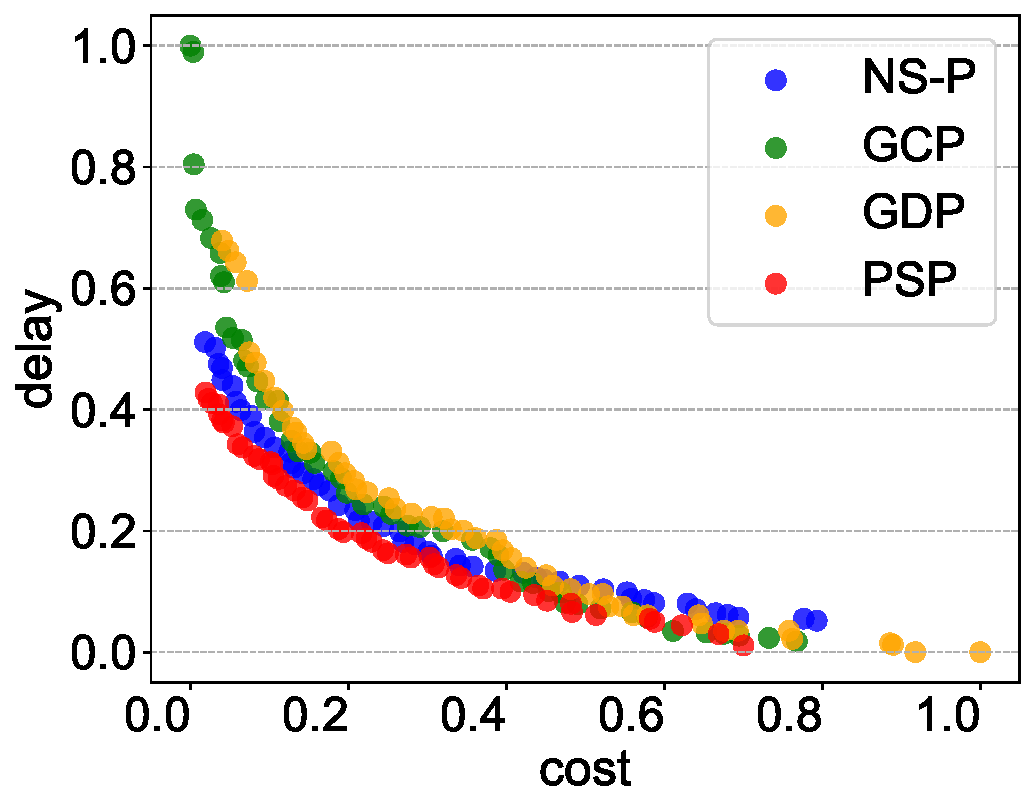
\includegraphics[width=1.73in]{nsga_data_5_130_new2.pdf}}
	\subfigure[\# edge servers (10).]
	{
\includegraphics[width=1.73in]{nsga_data_10_130_new2.pdf}}
	\subfigure[\# edge servers (15).]
	{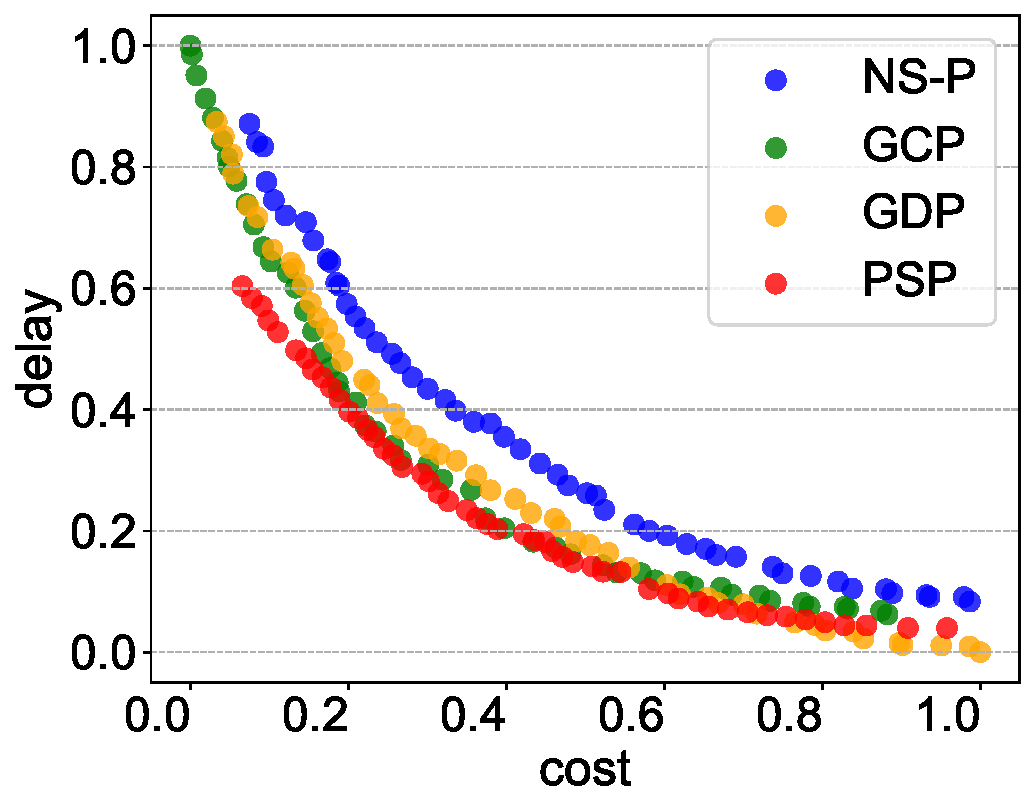
\includegraphics[width=1.73in]{nsga_data_15_130_new2.pdf}}
	\subfigure[\# edge servers (20).]
	{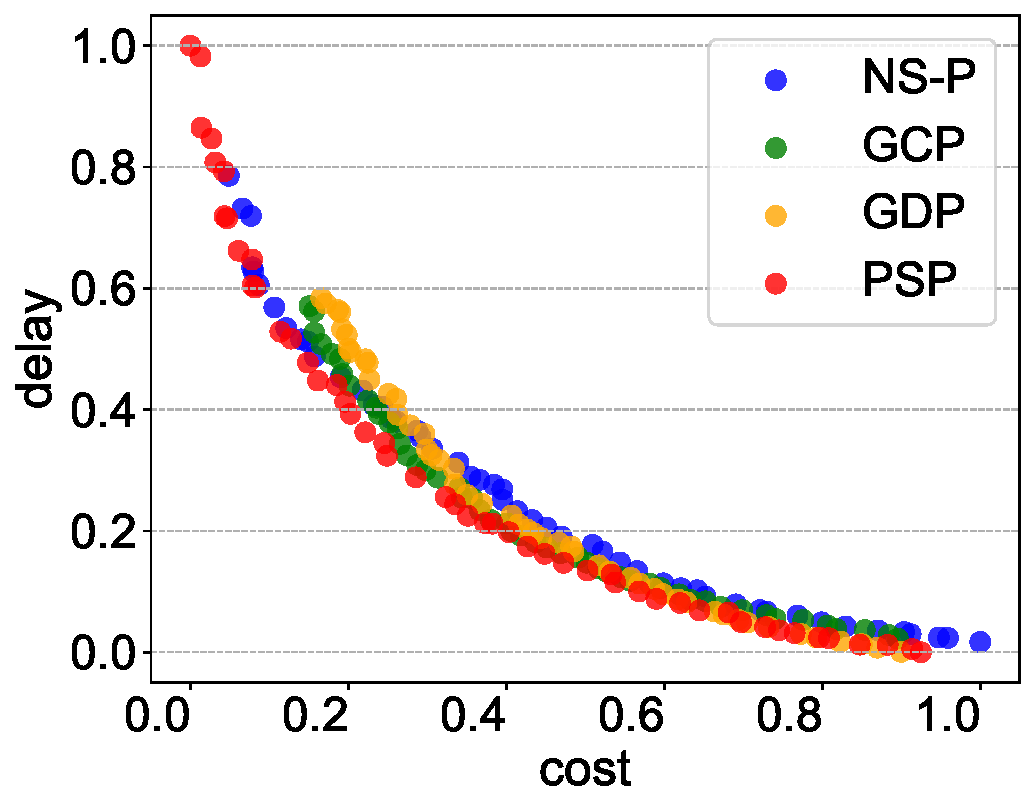
\includegraphics[width=1.73in]{nsga_data_20_130_new2.pdf}}
	\caption{Pareto fronts for Stage-II service provisioning with 130 users.}
	\label{fig7}
    \vspace{-7pt}
\end{figure*}


%\subsection{实验设置}

% 为了评估我们提出的 CLS 与 PSP 算法的性能表现，本文选取了来自中国电信公司的真实数据集，并将基站位置设定在北京市西直门地铁站附近约9千米的区域。在进行对比实验时，我们分别固定基站数量和用户规模，以验证在不同数据下算法的优越性。
% 在系统参数设置方面，每个服务器的覆盖范围设定为 1.5 千米，计算能力从 2GHz 到 5GHz，存储容量从 5GB 到 10GB，通信带宽在 300MB/s 到 1000MB/s 之间。每位用户均发出一项特定类别的服务请求，且每类服务拥有固定的部署成本与资源消耗要求。所有实验均在一台搭载 Windows 11 操作系统的工作站上完成，硬件配置包括 AMD Ryzen 7 5800H with Radeon Graphics 处理器，以及 NVIDIA GeForce RTX 3050 Ti GPU，并配备 32GB 内存。
%%%new:
To evaluate the performance of our proposed CLS and PSP algorithms, we utilized a dataset obtained from China Telecom Company, with base station locations set within approximately a 9 km radius around Xizhimen Subway Station in Beijing. For the comparative experiments, we sequentially fixed the number of base stations and the scale of user requests to verify the effectiveness and superiority of the proposed algorithms under different data configurations. 
Regarding the system configuration, each server was assigned a coverage radius of 1.5 km, with computational capacities ranging from 2 GHz to 5 GHz, storage sizes from 5 GB to 10 GB, and communication bandwidths between 300 MB/s and 1000 MB/s. Each user submitted a service request belonging to a specific category, where each service type has fixed deployment costs and resource requirements. All experiments were conducted on a workstation running Windows 11, equipped with an AMD Ryzen 7 5800H with Radeon Graphics processor, an NVIDIA GeForce RTX 3050 Ti GPU, and 32 GB of RAM.


The evolutionary settings used for PSP are summarized in Table~\ref{tab:psp_parameters}. The deterministic anchor size is defined proportionally as $\varpi_j=\lceil\rho V_j\rceil$ with $\rho=0.5$. Hence, for the experimental capacity $V_j=4$, two slots retain the highest-scoring services and two slots preserve stochastic exploration. This equal allocation provides an interpretable exploitation--exploration balance and applies directly to servers with different capacities.

For each server/user configuration, cost and delay are normalized over the pooled solutions of the compared methods as
\begin{equation}
\widehat{C}=\frac{C-C_{\min}}{C_{\max}-C_{\min}},\qquad
\widehat{D}=\frac{D-D_{\min}}{D_{\max}-D_{\min}},
\label{eq:q_normalization}
\end{equation}
and the scalar evaluation score is
\begin{equation}
Q=\lambda\widehat{C}+(1-\lambda)\widehat{D},\qquad \lambda=0.5.
\label{eq:q_score}
\end{equation}
Lower $Q$ indicates a better balanced solution. Hypervolume (HV) measures the dominated objective-space volume relative to the reference point $(1.1,1.1)$ and is maximized, whereas inverted generational distance (IGD) measures the mean distance from the common non-dominated reference front to a method's front and is minimized.


\begin{table}[!t]
\centering

\caption{NSGA-II and PSP parameter settings.}
\label{tab:psp_parameters}
\small
\begin{tabular}{|l|c|}
\hline
Parameter & Value \\ \hline
Population size $N$ & 50 \\ \hline
Maximum generations $G$ & 200 \\ \hline
SBX crossover & $p_c=0.9$, $\eta_c=15$ \\ \hline
Polynomial mutation & $p_m=1/(k|\mathcal{S}|)$, $\eta_m=20$ \\ \hline
Hybrid-score weights & $\alpha=\beta=0.5$ \\ \hline
Service capacity & $V_j=4$ \\ \hline
Anchor ratio & $\rho=0.5$ \\ \hline
\end{tabular}
\end{table}

% The hyperparameters used in the Algorithms \ref{algo:interior_point} and \ref{algo:branch_and_bound} are summarized in Table~\ref{tab: hyperparameters}.
% \begin{table}[!t]
% \centering
% \caption{parameters and Values}
% \label{tab: hyperparameters}
% \begin{tabular}{|c|c|}
% \hline
% parameter & Value \\
% \hline
% $\alpha$ & 0.6 \\
% $\gamma$ & 0.7 \\
% $\omega$ & 50 \\
% $\varepsilon$ & $10^{-6}$ \\
% $\rho$ & 0.1 \\
% \hline
% \end{tabular}
% \end{table}

In Stage~I, CLS is compared with four baseline methods:
%Local-Search对比算法
\begin{itemize}
    \item \textbf{Random Deployment (RD)}: $k$ base stations are randomly selected as edge server deployment locations.
    \item \textbf{Density Based Deployment (DBD)}: Base stations are ranked by user density within their coverage areas, and the top-$k$ locations are selected for edge server deployment.
    \item \textbf{Distance-Sum Deployment (DSD)}: For each base station, the cumulative distance to all users is computed, and the top-$k$ locations with minimal total distance are chosen for edge server deployment.
    \item \textbf{Greedy-K Deployment (GKD)}: The algorithm iteratively selects base stations that maximize the reduction in total user distance until $k$ servers are deployed.
\end{itemize}


In Stage~II, PSP is compared with four baseline strategies:

%NSGA-II对比算法
\begin{itemize}
    \item \textbf{NSGA-II Provision (NS-P)}: The initial population is generated randomly.
    \item \textbf{Greedy-Cost Provision (GCP)}: Services with the lowest deployment costs are prioritized until the capacity limit is reached during initial population generation.
    \item \textbf{Greedy-Delay Provision (GDP)}: Services with the highest request volumes are prioritized until the capacity limit is reached during initial population generation to minimize user delay.
    \item \textbf{Deep Q-Network Provision (DQN)}: A Q-network sequentially selects a service or an empty action for each server slot using demand, deployment cost, and a cost--delay preference. The resulting deployment is evaluated by the same objectives as the other methods.
\end{itemize}

\subsection{Experiment Results}
\subsubsection{Stage I: Server Deployment}

To examine the effect of the initial deployment set in Algorithm~\ref{algo:local_search}, we compare Random, Density, DistSum, marginal Greedy, and Diverse initialization over 50 runs. For each configuration, the reported gap is the percentage difference between the final cost and the best final cost observed under the same server/user setting. As shown in Fig.~\ref{fig:cls_init}, the five strategies reach the same best final cost in nearly all fixed-130-user cases; the only nonzero entry is the 2.10\% mean gap of Random at 10 servers. Under the 10-server/150-user setting, Random obtains a 1.27\% mean gap, whereas marginal Greedy reaches 15.88\%. These results show that CLS is generally stable across initializations and that random initialization avoids a systematic preference for a poorer local optimum.


\begin{figure}[!t]
    \centering
    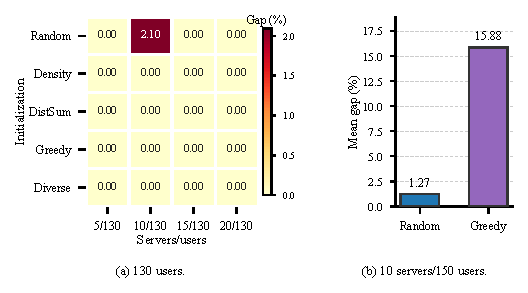
\includegraphics[width=\columnwidth]{cls_initialization_sensitivity_compact.pdf}
    \caption{Initialization sensitivity of CLS under two server/user settings.}
    \label{fig:cls_init}
\end{figure}
%对于stage 1,我们设计了两组实验来证明该放置策略的优越性。
%首先，在确定放置个数时，我们会选取确定的k值，k±2以及放置个数上限N_1共6个值分别代入计算服务器放置成本和通讯成本的模型进行求解，得出在对应服务器数量取值下经过局部搜索求解后产生的对应成本。经过实验结果Fig 3(a)可以看出，本策略确定的k值在与其附近的值对比后仍具有最低的成本消耗，在实现了优化服务器放置成本的同时，还可以在不同服务器放置数量下优化通讯成本。Fig 3(b)表示当k为10时，经过多轮迭代，算法逐渐达到最优状态，最终收敛，通讯成本也随之优化。
%其次，为了验证CLP算法的优越性，我们分别选取10和20个服务器进行放置，仿真180和300个用户坐标进行对比实验。Fig 6(a)展示了不同算法在不同基站数量、不同用户数量下的通讯成本比较。随着数据规模的变化，可以观察到 CLS 算法始终保持较低的通讯成本；而其他算法的通讯成本普遍较高。值得注意的是，DSD和GKD在用户集合和基站规模的程度增大到一定程度后成本显著提高，可能是因为在大规模数据中算法过度看中用户距离的影响而忽略的用户密度的分布，算法可能会因为适应某几个距离特别偏远的用户从而忽视其他距离更近、分布更多的用户，而局部搜索策略由于存在多轮迭代，尽量避免了这种情况，证明其策略具有优越性。
We design two sets of experiments to demonstrate the superiority of our deployment strategy. 

First, when determining the optimal number of servers $k$, we evaluate six values: the optimal $k$, $k \pm 2$, and the maximum deployment capacity $\mathcal{K}^c$. These values are input into our cost model that jointly optimizes server deployment cost and communication cost. As shown in Fig.~\ref{fig_compare}(a), our strategy achieves the lowest cost consumption at the determined $k$ compared to neighboring values, demonstrating simultaneous optimization of both deployment and communication costs across varying server counts. Furthermore, Fig.~\ref{fig_compare}(b) illustrates the convergence behavior when $k=10$, where the algorithm progressively reaches optimal states through multiple iterations, resulting in optimized communication costs.

Second, to validate the superiority of our CLS algorithm, we conduct comparative experiments deploying 10 and 20 servers to serve 180 and 300 users, respectively. Fig.~\ref{fig2} presents the communication cost comparison across different algorithms under varying base station and user scales, revealing two critical findings: (1) the CLS algorithm consistently maintains lower communication costs as data scales increase, while (2) other algorithms—particularly DSD and GKD—exhibit significantly higher costs when user/base station scales exceed certain thresholds. This degradation occurs because DSD and GKD overemphasize user distance metrics while neglecting density distribution, adapting to distant outliers at the expense of clustered nearby users. In contrast, our local search strategy mitigates this issue through iterative optimization, demonstrating superior robustness in large-scale scenarios.

\subsubsection{Stage II: Service Provisioning}
%对于stage 2,我们通过比较不同规模的基站数量和用户数量来验证本文经过改进的PSP策略具有优越性。
%我们分别将放置的服务器数量固定为10，将用户数量从100依次增加到180；以及将用户数量固定为130，放置服务器数量从5依次增加到20。Fig3,Fig4为两组对比实验的效果图，纵坐标为部署成本与用户延迟的归一化加权总开销。从图中可以看出，PSP策略的加权值始终为最低。由于GCP、GDP分别对算法的初始种群生成做出了一定的优化，因此其效果普遍优于NS-P的原始随机生成初始种群的策略。而PSP在对GCP、GDP的初始种群选取部分解进行结合的同时，又加入了一定随机性使其避免陷入局部最优的情况，因此往往能得出优化效果最好的解。
%Fig5展示了其中一组固定用户数量130，逐渐增加服务器数量的对比实验的帕累托解集。从图中可以看出，红色曲线（PSP）在大部分情况下的覆盖率都优于其他三种策略的曲线，表明在同一种优化倾向的情况下，PSP策略对部署成本和用户延迟的优化程度总是比其他策略更好。因此，本阶段的实验证明我们提出的PSP策略的联合优化程度最显著，具有优越性。

We evaluate Stage~II under two complementary configurations: (i) 10 deployed servers with 100, 130, 150, and 180 users, and (ii) 130 users with 5, 10, 15, and 20 deployed servers. Figures~\ref{fig4} and~\ref{fig6} report the minimum normalized score $Q$ obtained by each method. PSP achieves the lowest $Q$ in every reported case across both experimental series. Its hybrid initialization consistently improves upon random NS-P and the single-criterion GCP and GDP initializations; PSP also achieves lower $Q$ than DQN across all tested scales.

Figure~\ref{fig7} compares the cost--delay fronts generated by the four NSGA-II-based provisioning strategies with 130 users. Table~\ref{tab:pareto_metrics} gives the numerical results for the 10-server setting. PSP attains the largest HV (0.9470), the smallest IGD (0.0016), and the smallest $Q$ (0.3282), confirming both broader objective-space coverage and closer convergence to the common reference front. DQN produces a limited set of scalarized solutions rather than a population-based Pareto front; it is therefore compared through $Q$ and is not included in the HV/IGD comparison.


\begin{table}[!t]
\centering

\caption{Pareto quality with 10 servers and 130 users.}
\label{tab:pareto_metrics}
\small
\begin{tabular}{|l|c|c|c|}
\hline
Method & HV $\uparrow$ & IGD $\downarrow$ & Best $Q$ $\downarrow$ \\ \hline
NS-P & 0.8191 & 0.0785 & 0.3894 \\ \hline
GCP  & 0.8596 & 0.0492 & 0.3550 \\ \hline
GDP  & 0.8945 & 0.0326 & 0.3363 \\ \hline
PSP  & \textbf{0.9470} & \textbf{0.0016} & \textbf{0.3282} \\ \hline
DQN  & -- & -- & 0.6125 \\ \hline
\end{tabular}
\end{table}

\section{Conclusion}
 This paper presents MOS², a two-stage multi-objective framework for joint cost-delay optimization in mobile edge networks,
   addressing server deployment and service provisioning in multi-user scenarios. In the first stage, we develop a
  Coverage-based Local Search (CLS) algorithm that determines the number of deployable servers from budget and user-density
  constraints and then iteratively refines their placement to minimize deployment and transmission cost. Building on the
  resulting spatial configuration, the second stage formulates service provisioning as a bi-objective problem and solves it
  with a Pareto-oriented Service Provisioning (PSP) strategy on top of NSGA-II. To accelerate convergence and improve
  solution quality, we further design a standalone Initial Base Configuration (IBC) procedure that fuses cost-oriented and
  delay-oriented greedy rankings into a structured initial seed, and we embed an explicit capacity-repair mechanism into the
   evolutionary loop to enforce feasibility. Complexity analyses are provided for both stages, and extensive experiments on
  real-world base station data show that the framework consistently outperforms baseline methods and delivers a rich set of
  Pareto-optimal trade-offs between cost and latency, giving network operators practical flexibility in provisioning
  decisions. Future work will extend the framework with reliability-aware QoS constraints for packet loss, link availability, and service interruption, together with learning-based demand prediction and multi-domain coordination.

% \section{CONCLUSION}
% In this paper, we investigate the problem of server deployment and service placement in a multi-user scenario, aiming to enhance the profits of MNOs while considering constraints related to distance thresholds, resource limitations, and connectivity requirements. We formulate a profit model to address the challenges of the problem. Based on that, we employ a two-stage method to decouple the problem, breaking it down into two distinct yet interconnected stages. On this basis, we proposed the SDQ and SPIB-TDB algorithms to effectively leverage time sequences with varying temporal validity for analysis. Finally, we conducted experiments using a real base station dataset provided by Shanghai Telecom to verify the superior performance of our proposed algorithms.

% \section*{Acknowledgment}
% This work is supported by the National Natural Science Foundation of China (62202019,62276011,61202076), and supported by the Beijing Municipal Natural Science Foundation (4192007), along with other government sponsors. The authors would like to thank the reviewers for their efforts and for providing helpful suggestions that have led to several important improvements in our work. We would also like to thank all teachers and students in our laboratory for helpful discussions.

\begin{thebibliography}{00}
\bibitem{b1} Wang S, Zhao Y, Xu J, et al. Edge server placement in mobile edge computing[J]. Journal of Parallel and Distributed Computing, 2019, 127: 160-168.
\bibitem{b2} Li Y, Wang S. An energy-aware edge server placement algorithm in mobile edge computing[C]//2018 IEEE International conference on edge computing (EDGE). IEEE, 2018: 66-73.

\bibitem{b3} Xu X, Xue Y, Qi L, et al. Load-aware edge server placement for mobile edge computing in 5G networks[C]//Service-Oriented Computing: 17th International Conference, ICSOC 2019, Toulouse, France, October 28–31, 2019, Proceedings 17. Springer International Publishing, 2019: 494-507.
\bibitem{b4} Jiang X, Hou P, Zhu H, et al. Dynamic and intelligent edge server placement based on deep reinforcement learning in mobile edge computing[J]. Ad Hoc Networks, 2023, 145: 103172.
\bibitem{b5} Kasi S K, Kasi M K, Ali K, et al. Heuristic edge server placement in industrial internet of things and cellular networks[J]. IEEE Internet of Things Journal, 2020, 8(13): 10308-10317.
\bibitem{b6} Wu J J, Shih S F, Liu P, et al. Optimizing server placement in distributed systems in the presence of competition[J]. Journal of Parallel and Distributed Computing, 2011, 71(1): 62-76.
\bibitem{b7} Shen B, Xu X, Qi L, et al. Dynamic server placement in edge computing toward internet of vehicles[J]. Computer Communications, 2021, 178: 114-123.

\bibitem{b8} Ling C, Feng Z, Xu L, et al. An edge server placement algorithm based on graph convolution network[J]. IEEE Transactions on Vehicular Technology, 2022, 72(4): 5224-5239.

\bibitem{b9} Luo F, Zheng S, Ding W, et al. An edge server placement method based on reinforcement learning[J]. Entropy, 2022, 24(3): 317.
\bibitem{b10} Zeng F, Ren Y, Deng X, et al. Cost-effective edge server placement in wireless metropolitan area networks[J]. Sensors, 2018, 19(1): 32.

%11-13是参考论文里的三篇
\bibitem{b11} Guo Y, Wang S, Zhou A, et al. User allocation-aware edge cloud placement in mobile edge computing[J]. Software: Practice and Experience, 2020, 50(5): 489-502.
\bibitem{b12} Xu Y, Chau V, Wu C, et al. Online joint placement and allocation of virtual network functions with heterogeneous servers[J]. IEEE Internet of Things Journal, 2020, 7(9): 8049-8058.
\bibitem{b13} Cui G, He Q, Chen F, et al. Trading off between user coverage and network robustness for edge server placement[J]. IEEE Transactions on Cloud Computing, 2020, 10(3): 2178-2189.

\bibitem{b14} Qian Y, Hu L, Chen J, et al. Privacy-aware service placement for mobile edge computing via federated learning[J].Information Sciences, 2019, 505: 562-570.

\bibitem{b15} Yu N, Xie Q, Wang Q, et al. Collaborative service placement for mobile edge computing applications[C]//2018 IEEE Global Communications Conference (GLOBECOM). IEEE, 2018: 1-6.

\bibitem{b16} Ma H, Zhou Z, Chen X. Predictive service placement in mobile edge computing[C]//2019 IEEE/CIC International Conference on Communications in China (ICCC). IEEE, 2019: 792-797.

\bibitem{b17} Ouyang T, Zhou Z, Chen X. Follow me at the edge: Mobility-aware dynamic service placement for mobile edge computing[J]. IEEE Journal on Selected Areas in Communications, 2018, 36(10): 2333-2345.
\bibitem{b18} Ouyang T, Li R, Chen X, et al. Adaptive user-managed service placement for mobile edge computing: An online learning approach[C]//IEEE INFOCOM 2019-IEEE conference on computer communications. IEEE, 2019: 1468-1476.
\bibitem{b19} Zhang Q, Zhu Q, Zhani M F, et al. Dynamic service placement in geographically distributed clouds[J]. IEEE Journal on Selected Areas in Communications, 2013, 31(12): 762-772.
\bibitem{b20} Skarlat O, Nardelli M, Schulte S, et al. Optimized IoT service placement in the fog[J]. Service Oriented Computing and Applications, 2017, 11(4): 427-443.
\bibitem{b21} Wang S, Urgaonkar R, He T, et al. Dynamic service placement for mobile micro-clouds with predicted future costs[J]. IEEE Transactions on Parallel and Distributed Systems, 2016,28(4): 1002-1016.
\bibitem{b22} Wang L, Jiao L, He T, et al. Service placement for collaborative edge applications[J]. IEEE/ACM Transactions on Networking, 2020, 29(1): 34-47.
\bibitem{b23} Cabrera C, Svorobej S, Palade A, et al. MAACO: A dynamic service placement model for smart cities[J]. IEEE Transactions on Services Computing, 2022, 16(1): 424-437.
\bibitem{b24} Yang L, Cao J, Liang G, et al. Cost aware service placement and load dispatching in mobile cloud systems[J]. IEEE Transactions on Computers, 2015, 65(5): 1440-1452.
\bibitem{b25} Chen L, Xu J, Ren S, et al. Spatio–temporal edge service placement: A bandit learning approach[J]. IEEE Transactions on Wireless Communications, 2018, 17(12): 8388-8401.
\bibitem{b26} Han P, Liu Y, Zhang X, et al. Energy-Efficient Service Placement Based on Equivalent Bandwidth in Cell Zooming Enabled Mobile Edge Cloud Networks[J]. IEEE Transactions on Vehicular Technology, 2022, 71(11): 12275-12290.
\bibitem{b27} Sami H, Mourad A, Otrok H, et al. Demand-driven deep reinforcement learning for scalable fog and service placement[J]. IEEE Transactions on Services Computing, 2021, 15(5): 2671-2684.
% \bibitem{b28} Li Y, Dai W, Gan X, et al. Cooperative service placement and scheduling in edge clouds: A deadline-driven approach[J]. IEEE Transactions on Mobile Computing, 2021, 21(10): 3519-3535.

\bibitem{b28} Lu S, Jin X, Wu J, et al. QoS-aware Dynamic Service Caching and Updating in Cost-efficient Multi-Access Edge Computing[C]//2024 IEEE International Symposium on Parallel and Distributed Processing with Applications (ISPA). IEEE, 2024: 1718-1725.

\bibitem{b29} Fang J, Wu S, Lu S, et al. Enhanced Profit-driven Optimization for Flexible Server Deployment and Service Placement in Multi-User Mobile Edge Computing Systems[J]. IEEE Transactions on Network Science and Engineering, 2024.

\bibitem{b30} Lu, S, Xiang, B, Wu, J, et al. Multi-Timescale Hierarchical Prefetching for Online Caching in Vehicular Edge Networks[C]. //In 2025 34th International Conference on Computer Communications and Networks (ICCCN) (pp. 1-9). IEEE.

\bibitem{b31} Lu S, Jin X, Wu J, et al. Enhanced Multi-Stage Optimization of Dynamic QoS-Aware Service Caching and Updating in Mobile Edge Computing[J]. IEEE Transactions on Network and Service Management, 2025.

\bibitem{b32} Liu, H, Xu, Z, Di, X, et al. Multi-Stage Pareto-Based Optimization for Joint Server Deployment and Service Provisioning in Mobile Edge Computing[C]. In 2025 IEEE International Symposium on Parallel and Distributed Processing with Applications (ISPA) (pp. 363-370). IEEE.

\bibitem{b33} C. Feng, M. Yang, Z. Jing, T. Q. S. Quek, and M. Mei, ``Latency-Aware Service Deployment and Peer Offloading: A Long-Term Optimization Framework for Satellite Edge Computing,'' IEEE Internet of Things Journal, vol. 13, no. 1, pp. 405--417, 2026.

\bibitem{b34} M. Kato, T. K. Rodrigues, and S. Verma, ``Novel Breakout Local Search for Offloading Tasks in Multi-Tiered Cloud Environment Considering Transmission and Processing,'' in Proc. 2025 9th IEEE International Conference on Network Intelligence and Digital Content (IC-NIDC), 2025, pp. 269--274.

\bibitem{b35} Z. Jing, Q. Yang, M. Qin, J. Li, and K. S. Kwak, ``Long-Term Max--Min Fairness Guarantee Mechanism for Integrated Multi-RAT and MEC Networks,'' IEEE Transactions on Vehicular Technology, vol. 70, no. 3, pp. 2478--2492, 2021.

\bibitem{b36} Z. Jing, X. Wang, Q. Yang, M. Mei, and Y. Wu, ``Dynamic Energy Cost Conservation for Distributed Edge Clouds Utilizing Online Mini-Batch Learning,'' in Proc. IEEE 34th Annual International Symposium on Personal, Indoor and Mobile Radio Communications (PIMRC), 2023, pp. 1--6.


\end{thebibliography}


\end{document}
